% !TeX spellcheck = en_US
% Time-stamp: <09/10/02 01:57:13 vilhuber>
% $Id: Presentation-UQAM20152015.tex 1764 2015-11-11 12:26:25Z lv39 $

% normal line:
\documentclass[xcolor=table,compress]{beamer}
% to create notes:
%\documentclass[handout,notes=only]{beamer}
% to create handouts
%\documentclass[xcolor=table,handout,compress]{beamer}
% to create a different kind of handouts
%\documentclass{article}
%\usepackage[envcountsect]{beamerarticle}

%\setbeameroption{handout}
%\setbeameroption{show notes}


%
% Packages
%
\mode<article> % only for the article version
{
  \usepackage{fullpage}
  \usepackage{hyperref}
}

\usepackage{ifpdf}
\ifpdf
\usepackage{embedfile}
\embedfile{\jobname.tex}
\fi

\usepackage{graphicx}
%\usepackage{pstricks}
\usepackage{xcolor}
\usepackage{pifont}
%\usepackage{../chicago}
\usepackage{pgf}
\usepackage{amsmath,amssymb,amsfonts}
\usepackage[latin1]{inputenc}
\usepackage{colortbl}
\usepackage[english]{babel}
\usepackage{array}
\usepackage{pdfpages}
\usepackage{wrapfig}


\usepackage{csvsimple}
\usepackage{tikz}
%\usetikzlibrary{shadows.blur}
\usetikzlibrary{shadows}
\usetikzlibrary{shapes.symbols}

\usepackage{calc}
\usepackage{algpseudocode}
\newenvironment{algorithm}{\begin{center}\hrule\ \\}{\hrule\end{center}}
\usepackage[printonlyused]{acronym}

% usage:
%   \includepdf[pages={1}]{myfile.pdf}
%   \includepdf[pages={1,3,5}]{myfile.pdf} would include pages 1, 3, and 5 of the file. 
%   To include the entire file, you specify pages={-}, where {-}
%\usepackage{landscape}

%\usepackage{lmodern}
%\usepackage[T1]{fontenc}

\usepackage{times}
\usepackage{transparent}
%\usepackage{colortbl}

%============================================================
% Beamer specific styles and configs
%============================================================

\mode<presentation>
{
% alternative, could always use
%\usetheme{Census}
\usetheme{cornell}
\useoutertheme{cornell}


% For Census template
%\usetheme{Malmoe}
%\usecolortheme{dove}
%\setbeamertemplate{background canvas}{\includegraphics
%        [height=\paperheight]{Census2014-background-4x3}}
%\setbeamertemplate{footline}[frame number]% page numbers and using Warsaw theme%
%\setbeamertemplate{navigation symbols}{}
}
%\setbeamercovered{dynamic}


%============================================================
% Title
%============================================================


\newcommand{\mytitle}{Using partially synthetic microdata to protect sensitive cells in business 
statistics}
\newcommand{\myshorttitle}{Partially Synthetic BDS}
\newcommand{\myversion}{\today}  %alternate version


\title[UQAM2015]{\mytitle}
\author[Vilhuber]{%
  Lars~Vilhuber\inst{1} 
}

\institute[Cornell]{
  \inst{1}%
   Labor Dynamics Institute,
  ILR, Cornell University, United States
%\and \inst{2} Center for Economic Studies, U.S. Census Bureau, United States
}%
\date[November 2015]{November 2015\\UQAM\\
Montr\'eal, Canada }
\subject{Synthetic Data; Establishment Microdata}

%
% Some useful commands
%

\newcommand{\rarrow}{\selectfont\ding{220}}
\newcommand{\skiplink}{\tiny{\gray\selectfont\ding{59}}}
\newcommand{\goback}{\Acrobatmenu{GoBack}{\gray\selectfont\ding{242}}}
\newcommand{\x}{\selectfont\ding{52}}
\newcommand{\verbatimsize}{\tiny}
\newcommand{\tablesize}{\footnotesize}

%
% The document proper
%
\begin{document}
%\transparent{0.9}
{
		\usebackgroundtemplate{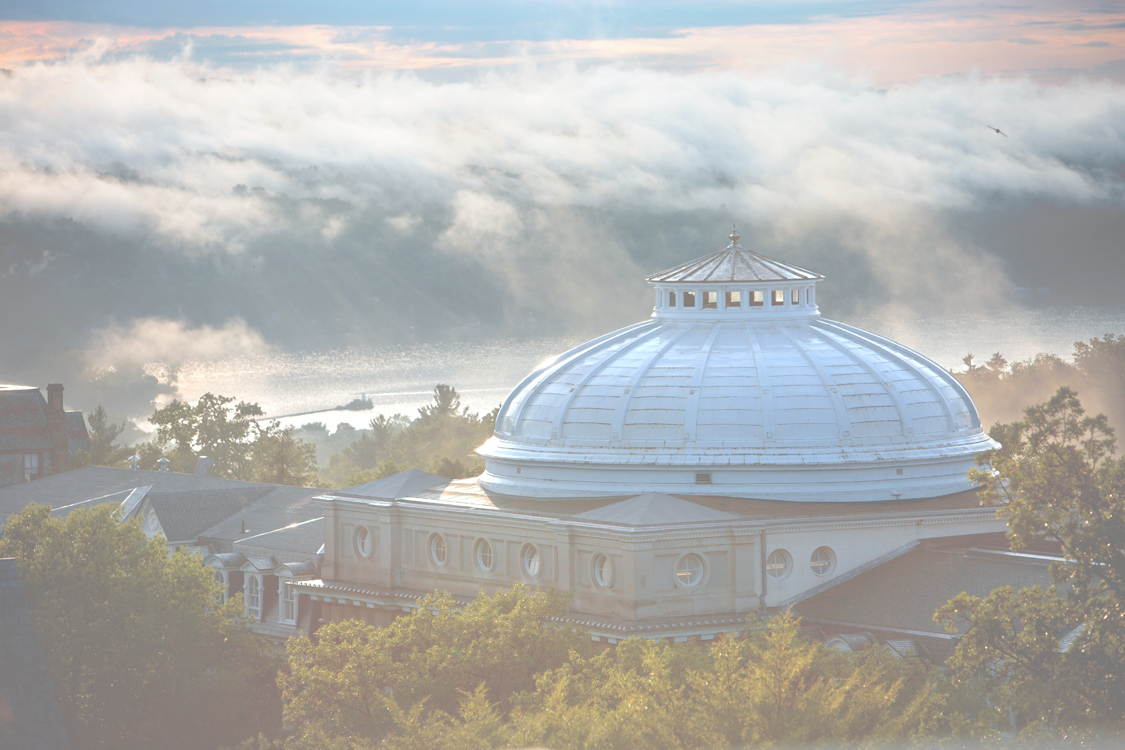
\includegraphics[width=\paperwidth]{2015_0795_015_transparent.png}}
\frame{\titlepage}
}
%\part<presentation>*{Outline}
%
%\begin{frame}
%  \frametitle{Outline}
%  \tableofcontents[part=1,pausesections]
%\end{frame}

% This puts the partial table of contents at the start of each subsection
%\AtBeginSubsection[]
%{
%  \begin{frame}<beamer>
%    \frametitle{Outline}
%    \tableofcontents[current,currentsubsection]
%  \end{frame}
%}
\AtBeginSection[]{
	\begin{frame}
		\vfill
		\centering
		\begin{beamercolorbox}[sep=8pt,center,shadow=true,rounded=true]{title}
			\usebeamerfont{title}\insertsectionhead\par%
		\end{beamercolorbox}
		\vfill
	\end{frame}
}
\part<presentation>{Main Talk}

%
%  From this point on, we should probably extract it to a sub-document
%

%TCIDATA{Version=5.00.0.2570}
%TCIDATA{LaTeXparent=0,0,Presentation-CAFE-displacement-subdoc.tex}
% $Id: Presentation-subdoc-disclaimer.tex 1764 2015-11-11 12:26:25Z lv39 $
% $URL: https://forge.cornell.edu/svn/repos/lv39_papers/BigThinkPresentations/UQAM2015/Presentation/Presentation-subdoc-disclaimer.tex $
\section{Disclaimer}
\begin{frame}
\begin{block}{Funding}
\begin{itemize}
\item Vilhuber's work is partially funded by NSF Grants 
\href{http://www.nsf.gov/awardsearch/showAward.do?AwardNumber=1042181}{\#1042181}, \href{http://www.nsf.gov/awardsearch/showAward.do?AwardNumber=1131848}{\#1131848},
and 
\href{http://www.nsf.gov/awardsearch/showAward.do?AwardNumber=0941226}{\#0941226}, and by a grant from the Alfred P. Sloan Foundation.

\end{itemize}
\end{block}
\begin{block}{Disclaimer}
\huge ``
\begin{quote}
\footnotesize This paper reports the results of research and analysis 
undertaken by Census Bureau staff. It has undergone a more limited review by the Census Bureau than its 
official publications. This report is released to inform interested parties and to encourage discussion. Any 
findings, conclusions or opinions are those of the authors. They do not necessarily reflect those of the Center for 
Economic Studies, the U.S. Census Bureau, or the National Science Foundation. 
\end{quote}
\flushright ''
\end{block}
\end{frame}


\begin{frame}{Acknowledgements}
\begin{block}{This work presents the results of collaborations with}
John Abowd, Bill Block, Warren Brown, Ben Perry, Carl Lagoze, Venky Kambhampaty, Ian Schmutte, Kevin McKinney, Javier Miranda, Flavio Stanchi, Hautahi Kingi, Ashwin Machanavajjhala, Mark Kutzbach, Matthew
Graham, Samuel Haney, and others.
\end{block}
\end{frame}


%%% Local Variables:
%%% mode: latex
%%% End:

\ifpdf
\embedfile{Presentation-subdoc-disclaimer.tex}
\fi


%TCIDATA{Version=5.00.0.2570}
%TCIDATA{LaTeXparent=0,0,Presentation-CAFE-displacement-subdoc.tex}
% $Id: Presentation-subdoc-access.tex 1766 2015-11-11 19:14:54Z lv39 $
% $URL: https://forge.cornell.edu/svn/repos/lv39_papers/BigThinkPresentations/UQAM2015/Presentation/Presentation-subdoc-access.tex $
\section{Context}


\begin{frame}
\frametitle{Economic analysis}
	\centering
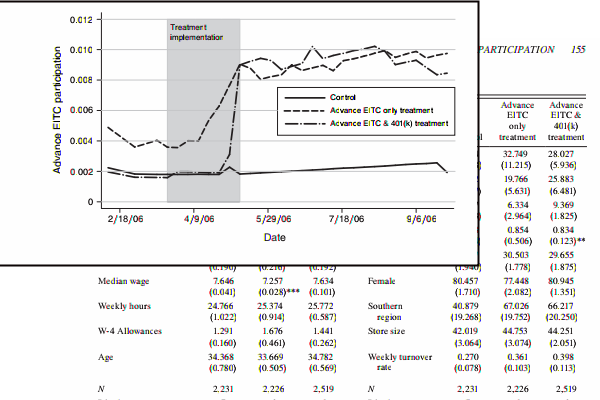
\includegraphics[width=0.9\textwidth]{Selection_119.png}
\end{frame}


\begin{frame}
\frametitle{The preponderance of public-use data}
\begin{block}{Microdata}
\begin{quote}
	``... paper uses data from the Current Population Survey...''
\end{quote}
\end{block}

\pause
\begin{block}{Macrodata}
	\begin{quote}
		``We use data downloaded from the Bureau of Economic Analysis...''
	\end{quote}
\end{block}

\end{frame}

% disaster: http://filmsplusmovies.com/wp-content/uploads/2013/08/Best-Natural-Disaster-Movies-Of-Hollywood.jpg

\begin{frame}
\centering
	
\includegraphics{temptation.jpg}% source:

	\tiny \href{http://www.bridgesofgraceucc.org/}{source} %http://www.bridgesofgraceucc.org/wp-content/uploads/2011/03/temptation.jpg
\end{frame}


\begin{frame}
\frametitle{Yielding...}
\begin{block}{Administrative data}
\begin{quote}
 ``Our analysis draws on administrative records from the Detroit Work First program
linked with unemployment insurance (UI) wage records for the State of
Michigan'' 

\tiny \href{http://doi.org/10.1257/app.2.3.96}{Autor/Houseman doi:10.1257/app.2.3.96}
\end{quote}
\end{block}
\pause
\begin{block}{Administrative data}
\begin{quote}
	``confidential student-level panel
dataset provided by the School Board of Alachua County in Florida'' 

\tiny \href{http://doi.org/10.1257/app.2.1.211}{Carrel and Hoekstra doi:10.1257/app.2.1.211}

\end{quote}\end{block}
\end{frame}


\begin{frame}
\frametitle{... yielding...}
\begin{block}{Proprietary data}
\begin{quote}
	``This field experiment was made possible by the collaboration of a large-scale,
	nationwide firm in the retail sector. ''
	
	\tiny \href{http://doi.org/10.1257/app.2.2.147}{Damon doi:10.1257/app.2.2.147}
\end{quote}
\end{block}
\end{frame}



\begin{frame}
\frametitle{The Death Knell for Public-use Data}

\centering
	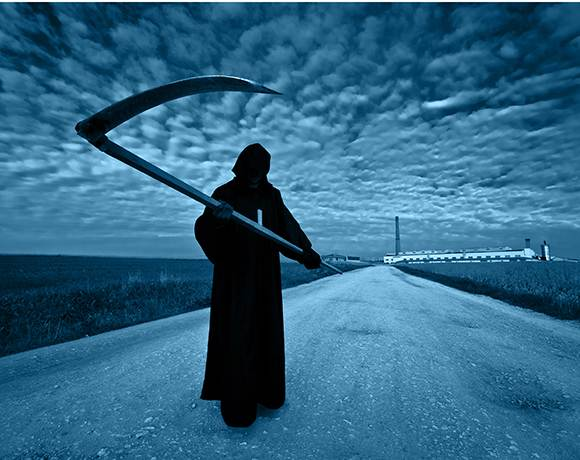
\includegraphics[width=.9\textwidth]{deathknell.jpg}% source: http://cdn.ttgtmedia.com/rms/onlineImages/ciomid_trends_2012_08.jpg

\end{frame}

\begin{frame}
	\frametitle{The Death Knell for Public-use Data}
\begin{itemize}
	\item Sounded by young scholars pursuing research
	programs that mandate inherently identifiable data:
			\begin{itemize}
				\item Geospatial relations,
				\item Exact genome data,
				\item Networks of all sorts,
				\item Linked administrative records
			\end{itemize}
			\item These researchers acquire authorized, generally unfettered, restricted access to the
			confidential, identifiable data and perform their analyses in secure
			environments.
\item But...

\end{itemize}
\end{frame}

\begin{frame}
%	\frametitle{The provenance problem}
	\begin{beamercolorbox}[sep=8pt,center]{title}
		\usebeamerfont{title} ...they don't leave behind the scientific trail that has
		made public-use files so important.
	\end{beamercolorbox}
\end{frame}


\begin{frame}
	\frametitle{Replication of research results}
	\begin{block}{Critical element of science}
		\begin{itemize}
			\item Replication of methods, data inputs, computational environment is a critical element of the scientific approach
			\item Journals, funding agencies (in the U.S.) have been moving to making archiving of inputs to scientific results more robust, even mandatory
		\end{itemize}
	\end{block}
\end{frame}


\begin{frame}
\frametitle{The problem}
\begin{block}{Good intentions, costly access}
\begin{quote}
	``researchers could submit programs that [...] research assistants
	would run. Alternatively, researchers wishing to work directly with the data could come and
	work on the Institute's premises. ''
\end{quote}
\end{block}
\pause
\begin{block}{Uncertain access}
\begin{quote}
	``Data [...] is proprietary and owned by the Alachua
County, Florida School District. The corresponding author [...] holds the deidentified
dataset [...] and will provide copies to
authors who receive written permission from the Alachua County Public Schools.''
\end{quote}
\end{block}
\pause
\begin{block}{No access}
\begin{quote}
	Some do not provide any information on access.	
\end{quote}
\end{block}
\end{frame}




\begin{frame}
	\frametitle{Not a new problem}
	\begin{columns}
	\begin{column}{.7\textwidth}
	\begin{block}{Econometrica}
		``In its first issue, the editor of Econometrica (1933), Ragnar Frisch, noted
		the importance of publishing data such that readers could fully explore
		empirical results.  Publication of data, however, was discontinued early in
		the journal's history.  [...]  The journal arrived full-circle in late 2004 when Econometrica
		adopted one of the more stringent policies on availability of data and
		programs.
	\end{block}
	\tiny \href{http://www.econometricsociety.org/submissions.asp\#4}{http://www.econometricsociety.org/submissions.asp\#4} as cited in \href{http://research.stlouisfed.org/wp/2005/2005-014.pdf}{Anderson et al (2005)}
	\end{column}
	\begin{column}{.3\textwidth}
\href{http://www.jstor.org/stable/i332704}{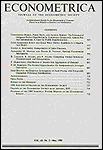
\includegraphics[width=\textwidth]{econometrica-vol1.png}}
	\end{column}
\end{columns}
\end{frame}

\begin{frame}
	\frametitle{Problem will become worse}
	\begin{block}{Increased use of restricted-access data}
\begin{itemize}
			\item Archiving (curation) of input data is complicated
			\item Knowledge discovery is complicated
		\end{itemize}
	\end{block}
\end{frame}
\begin{frame}
	\frametitle{Decline in the use of classic public-use data}
	\centering
	%\includepdf[pages={1-2}]{Chetty-1-2-Slides.pdf}
	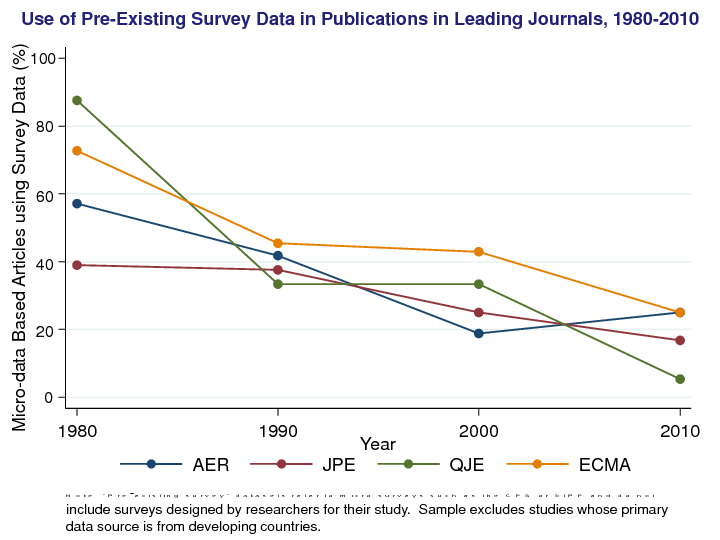
\includegraphics[width=0.7\paperwidth]{ChettySlide1}
\end{frame}

\begin{frame}
	\frametitle{Increase in the use of administrative data in economics}
	\centering
	%\includepdf[pages={1-2}]{Chetty-1-2-Slides.pdf}
	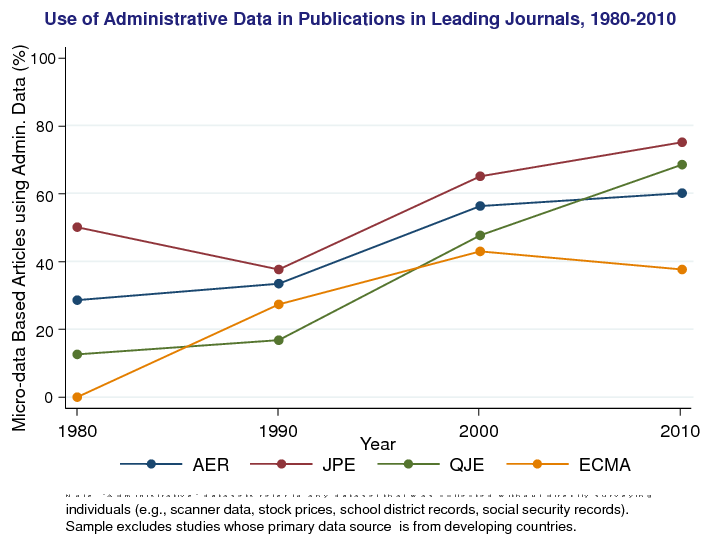
\includegraphics[width=0.7\paperwidth]{ChettySlide2}
\end{frame}


\begin{frame}
\frametitle{Results from the LDI Replication Lab}
	\begin{block}{Undergraduate research team}
		\begin{itemize}
			\item Census of articles in the American Economic Journal: Applied Economics (2010, 2011, 2013)
			\item Each article is analyzed for availability of replication archive (as required by journal!) 
			\item If data and programs are available, reproducibility is tested. 
		\end{itemize}
	\end{block}
\end{frame}

% extract from Replication.Rnw

\begin{frame}
\frametitle{Some very preliminary results}
	
	\centering
	\begin{table}[!htbp] \centering 
		\caption{Replication Success} 
		\label{} 
		\begin{tabular}{@{\extracolsep{5pt}} ccccc} 
			\\[-1.8ex]\hline 
			\hline \\[-1.8ex] 
			& Yes & No & Partial & Sum \\ 
			\hline \\[-1.8ex] 
			2010 & $10$ & $19$ & $6$ & $35$ \\ 
			2011 & $12$ & $20$ & $4$ & $36$ \\ 
			2013 & $15$ & $12$ & $11$ & $38$ \\ 
			\hline \\[-1.8ex] 
			
			\bf		Total &\bf $37$ &\bf $51$ &\bf $21$ &\bf $109$ \\ 
			\hline \\[-1.8ex] 
		\end{tabular} 
	\end{table} 
\end{frame}

\begin{frame}
\frametitle{Some very preliminary results}
	% Table created by stargazer v.5.2 by Marek Hlavac, Harvard University. E-mail: hlavac at fas.harvard.edu
	% Date and time: Mon, Nov 09, 2015 - 09:22:20 PM
	\centering \small
	\begin{table}[!htbp] 
		\caption{Reason for Replication Failure} 
		\label{} 
		\begin{tabular}{@{\extracolsep{5pt}} cccccc} 
			\\[-1.8ex]\hline 
			\hline \\[-1.8ex] 
			& Missing  & Corrupted  & Code  & Missing &  \\ 
			& Data     & Data       & Error & Code    & Sum \\ 
			\hline \\[-1.8ex] 
			2010 & $15$ & $1$ & $1$ & $2$ & $19$ \\ 
			2011 & $15$ & $1$ & $1$ & $3$ & $20$ \\ 
			2013 & $12$ & $0$ & $0$ & $0$ & $12$ \\ 
			\hline \\[-1.8ex] 
			\bf Total &\bf $42$ &\bf $2$ &\bf $2$ &\bf $5$ &\bf $51$ \\ 
			\hline \\[-1.8ex] 
		\end{tabular} 
	\end{table} 
\end{frame}


\begin{frame}
\frametitle{Some very preliminary results}
	\centering
	% Table created by stargazer v.5.2 by Marek Hlavac, Harvard University. E-mail: hlavac at fas.harvard.edu
	% Date and time: Tue, Nov 10, 2015 - 01:24:18
	\begin{table}[!htbp] \centering 
		\caption{Reason for Missing Data} 
		\label{} 
		\begin{tabular}{ ccccccc} 
			\\[-1.8ex]\hline 
			\hline \\[-1.8ex] 
		&\multicolumn{3}{c}{Administrative}&\multicolumn{2}{c}{Private} &  \\ 
		\cline{2-4}\cline{5-6}
		&  local &  National &  Regional &  Commercial &  Other & Sum \\ 
		\hline \\[-1.8ex] 
		2010 & $2$ & $8$ & $0$ & $4$ & $3$ & $17$ \\ 
		2011 & $2$ & $8$ & $4$ & $1$ & $0$ & $15$ \\ 
		2013 & $2$ & $2$ & $1$ & $4$ & $2$ & $11$ \\ 
			\hline \\[-1.8ex] 
		Total & $6$ & $18$ & $5$ & $9$ & $5$ & $43$ \\ 
			\hline \\[-1.8ex] 
		\end{tabular} 
	\end{table} 
\end{frame}


\begin{frame}
	\frametitle{Some very preliminary results}
% Table created by stargazer v.5.2 by Marek Hlavac, Harvard University. E-mail: hlavac at fas.harvard.edu
% Date and time: Tue, Nov 10, 2015 - 01:24:18
\begin{table}[!htbp] \centering 
	\caption{Type of Access to Confidential Data} 
	\label{} 
	\begin{tabular}{ cccccc} 
		\\[-1.8ex]\hline 
		\hline \\[-1.8ex] 
		&  &\multicolumn{2}{c}{Informal} & No  &  \\ 
		& Formal & w/ Commitment & w/o Commitment &  Info & Sum \\ 
		\hline \\[-1.8ex] 
		2010 & $2$ & $3$ & $9$ & $3$ & $17$ \\ 
		2011 & $2$ & $0$ & $10$ & $3$ & $15$ \\ 
		2013 & $1$ & $2$ & $8$ & $0$ & $11$ \\ 
		\hline \\[-1.8ex] 
	\bf	Total & $5$ & $5$ & $27$ & $6$ & $43$ \\ 
		\hline \\[-1.8ex] 
	\end{tabular} 
\end{table} 
		\end{frame}



\begin{frame}
	\frametitle{Not limited to one journal}
	\begin{block}{NIH-funded research}
		\begin{itemize}
			\item article is open-access
			\item not clear about data access
		\end{itemize}
	\end{block}
\end{frame}

  \tikzset{
  	arr/.style={->,blue,very thick},
  	lbl/.style={draw,blue,very thick},
  	shadowed/.style={preaction={transform canvas={shift={(2pt,-1pt)}},draw=gray,very thick}},
}
\begin{frame}
	\frametitle{A small anonymous example}
   \begin{tikzpicture}
   \node[draw=none,drop shadow={shadow scale=0.97,
   top color=black,bottom color=gray,
                          shadow xshift=3pt,
                          shadow yshift=-2pt,
   opacity=0.9}]
    at (1,1) {\fcolorbox{black}{white}{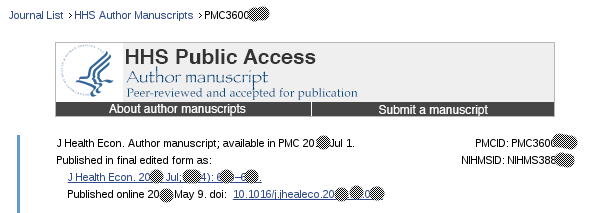
\includegraphics[scale=0.5]{Selection_031}}}; \pause
%
      \node[draw=none,drop shadow={shadow scale=0.95,
      	top color=black,bottom color=gray,
      	shadow xshift=3pt,
      	shadow yshift=-2pt,
      	opacity=0.9}]
      at (1,1) {\fcolorbox{black}{white}{
\includegraphics[scale=0.5]{Selection_030}}};
\pause
      \node[draw=none,drop shadow={shadow scale=0.93,
      	top color=black,bottom color=gray,
      	shadow xshift=3pt,
      	shadow yshift=-2pt,
      	opacity=0.9}]
      at (1,1) {\fcolorbox{black}{white}{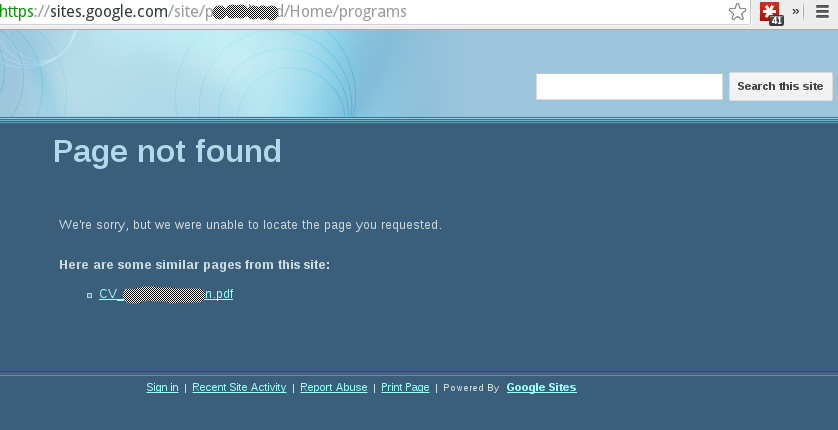
\includegraphics[scale=0.25]{Selection_032}}};
\pause
\node[draw=none,drop shadow={shadow scale=0.93,
	top color=black,bottom color=gray,
	shadow xshift=3pt,
	shadow yshift=-2pt,
	opacity=0.9}]
at (1,1) {\fcolorbox{black}{white}{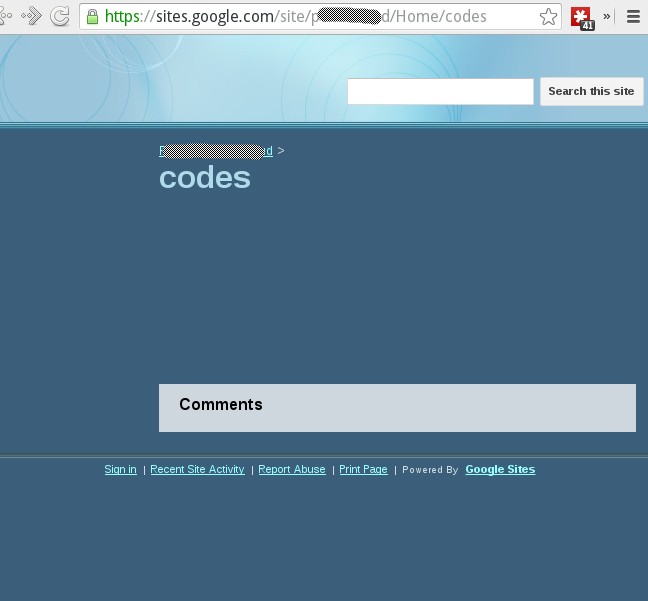
\includegraphics[scale=0.25]{Selection_029}}};
   \end{tikzpicture}

\end{frame}

\begin{frame}
	\frametitle{Not limited to economics}
	\begin{block}{Nature, 2012}
		``Many of the emerging `big data' applications come from private sources that are inaccessible to other researchers. The data source may be hidden, compounding problems of verification, as well as concerns about the generality of the results.''\\
	\end{block}
	{\tiny (Huberman, Nature 482, 308 (16 February 2012) \href{http://dx.doi.org/10.1038/482308d}{doi:10.1038/482308d})}
	\begin{block}{Other domains}
		\begin{itemize}
			\item Biology (genetics data, chemical compounds)
			\item Computer science (search records, single-firm examples)
		\end{itemize}
	\end{block}
\end{frame}


\begin{frame}
	\centering
	
\includegraphics[width=\textwidth]{Best-Natural-Disaster-Movies-Of-Hollywood.jpg}
\end{frame}



\begin{frame}
\frametitle{A program}
%\begin{block}{Broadening access}
%	\begin{itemize}
%		\item Public-use data is the ultimate decentralized computation
%		\item Current limits of the infrastructure
%		\item Infrastructure
%	\end{itemize}
%\end{block}


\begin{block}{Allowing for easier documentation of provenance}
\begin{itemize}
	\item Better documentation about confidential data
	\item Solving the reproducibility problem
\end{itemize}
\end{block}

\begin{block}{Making data more accessible}
	\begin{itemize}
		\item New disclosure limitation techniques
		\item New data access models
	\end{itemize}
\end{block}
\end{frame}


%%% Local Variables:
%%% mode: latex
%%% End:

\ifpdf
\embedfile{Presentation-subdoc-access.tex}
\fi

%TCIDATA{Version=5.00.0.2570}
%TCIDATA{LaTeXparent=0,0,Presentation-CAFE-displacement-subdoc.tex}
% $Id: Presentation-subdoc-replicability.tex 1765 2015-11-11 12:50:51Z lv39 $
% $URL: https://forge.cornell.edu/svn/repos/lv39_papers/BigThinkPresentations/UQAM2015/Presentation/Presentation-subdoc-replicability.tex $
\section{Replicability}


\begin{frame}
	\frametitle{Non-federal confidential data}
	States, school districts, private companies, academic and private surveys: need a place to live to be re-used.
	\begin{block}{Options}
		\begin{itemize}
			\item openICPSR \url{https://www.openicpsr.org/}
			\item Harvard Dataverse \url{https://dataverse.harvard.edu/} {\footnotesize (1,315\ DV, 59,530 DS)}
			\item Ontario Council of University Libraries: \url{http://dataverse.scholarsportal.info/dvn/} {\footnotesize (64\ DV, 5,289 files)}
		\end{itemize}
	\end{block}
	Hinges on compatibility of data deposit rules, laws, regulations, etc.
\end{frame}


\begin{frame}
	\frametitle{Can we influence this process?}
	\begin{block}{Data repositories have the technology to receive deposits}
		\begin{itemize}
			\item Underutilized
			\item When integrated into journal workflows, useless (blobs of unstructured ZIP files)
		\end{itemize}
	\end{block}
	\begin{block}{Journals can require data citations}
		\begin{itemize}
			\item Review process scrutinizes \textit{article} citations
			\item Would be easy to enforce \textit{data} citations
		\end{itemize}
	\end{block}
\end{frame}

\begin{frame}
	\frametitle{Data citations}
	\begin{block}{Examples} {\tiny  \footnotesize \tt
		\begin{quote}
			Deschenes, Elizabeth Piper, Susan Turner, and Joan Petersilia. \textbf{Intensive Community Supervision in Minnesota, 1990-1992: A Dual Experiment in Prison Diversion and Enhanced Supervised Release} [Computer file]. ICPSR06849-v1. Ann Arbor, MI: Inter-university Consortium for Political and Social Research [distributor], 2000. \alert<2>{doi:10.3886/ICPSR06849}
		\end{quote}
		\begin{quote}
			Abowd, John M.; Vilhuber, Lars, 2014, "\textbf{Replication data for: National estimates of gross employment and job flows from the Quarterly Workforce Indicators with demographic and industry detail}", \alert<2>{doi:10.7910/DVN/27923}, Harvard Dataverse [Distributor], V2
		\end{quote}[\href{http://www.icpsr.umich.edu/icpsrweb/ICPSR/curation/citations.jsp}{src}]}
	\end{block}
\end{frame}

\begin{frame}
	\frametitle{So we know how to deposit and cite data...}
	\pause
\begin{beamercolorbox}[sep=8pt,center]{title}
	\usebeamerfont{title}... except nobody does it...
\end{beamercolorbox}

\end{frame}

\begin{frame}
	\frametitle{We didn't do it...}
	\begin{block}{Abowd and Vilhuber (2011)}
   \begin{tikzpicture}
   \node[draw=none,drop shadow={shadow scale=0.97,
   	top color=black,bottom color=gray,
   	shadow xshift=3pt,
   	shadow yshift=-2pt,
   	opacity=0.9}]
   at (1,1) {\fcolorbox{black}{white}{
\includegraphics[scale=0.5]{Selection_126}}}; \pause
   %
   \node[draw=none,drop shadow={shadow scale=0.95,
   	top color=black,bottom color=gray,
   	shadow xshift=3pt,
   	shadow yshift=-2pt,
   	opacity=0.9}]
   at (1,1) {\fcolorbox{black}{white}{
\includegraphics[scale=0.5]{Selection_125}}};
   \pause
   \node[draw=none,drop shadow={shadow scale=0.93,
   	top color=black,bottom color=gray,
   	shadow xshift=3pt,
   	shadow yshift=-2pt,
   	opacity=0.9}]
   at (1,1) {\fcolorbox{black}{white}{
\includegraphics[scale=0.5]{Selection_124}}};
   \end{tikzpicture}		
	\end{block}
\end{frame}

\begin{frame}
	\frametitle{Then we archived it better...}
	\begin{block}{... at Harvard Dataverse}
   \begin{tikzpicture}
   \node[draw=none,drop shadow={shadow scale=0.97,
   	top color=black,bottom color=gray,
   	shadow xshift=3pt,
   	shadow yshift=-2pt,
   	opacity=0.9}]
   at (1,1) {\fcolorbox{black}{white}{
\includegraphics[scale=0.3]{Selection_128}}}; \pause
   %
   \node[draw=none,drop shadow={shadow scale=0.95,
   	top color=black,bottom color=gray,
   	shadow xshift=3pt,
   	shadow yshift=-2pt,
   	opacity=0.9}]
   at (1,1) {\fcolorbox{black}{white}{
\includegraphics[scale=0.3]{Selection_129}}};\pause
   %
   \node[draw=none,drop shadow={shadow scale=0.95,
   	top color=black,bottom color=gray,
   	shadow xshift=3pt,
   	shadow yshift=-2pt,
   	opacity=0.9}]
   at (1,1) {\fcolorbox{black}{white}{
\includegraphics[scale=0.3]{Selection_129_hilight}}};
   \end{tikzpicture}		
	\end{block}
\end{frame}

\begin{frame}{Provenance}
	\begin{block}{The provenance problem}
		``data provenance, one kind of metadata, pertains to the derivation history of a
		data product starting from its original sources'' [...]  ``from it, one can ascertain
		the quality of the data base and its ancestral data and derivations, track back sources
		of errors, allow automated reenactment of derivations to update the data, and provide 
		attribution of data sources'' 
	\end{block}
	{\tiny Simmhan, Plale, and Gannon, ``A survey of data provenance in e-science,'' ACM Sigmod Record, 2005}
\end{frame}


\begin{frame}{Provenance (cont)}
	\begin{block}{PROV model}
		W3C PROV Model  based in the notions of 
		\begin{enumerate}
			\item \textbf{entities} that are physical, digital, and conceptual
			things in the world; 
			\item \textbf{activities} that are dynamic aspects of the world that change and
			create entities; and 
			\item \textbf{agents} that are responsible for activities. 
			\item  a set of \textbf{relationships} that can exist be-
			tween them that express attribution,. delegation, derivation, etc.
		\end{enumerate}
	\end{block}
	\begin{block}{PROV and Metadata}
		Not (currently) a ``native'' component of DDI
	\end{block}
\end{frame}

\begin{frame}{Incorporating PROV (LBD)}
	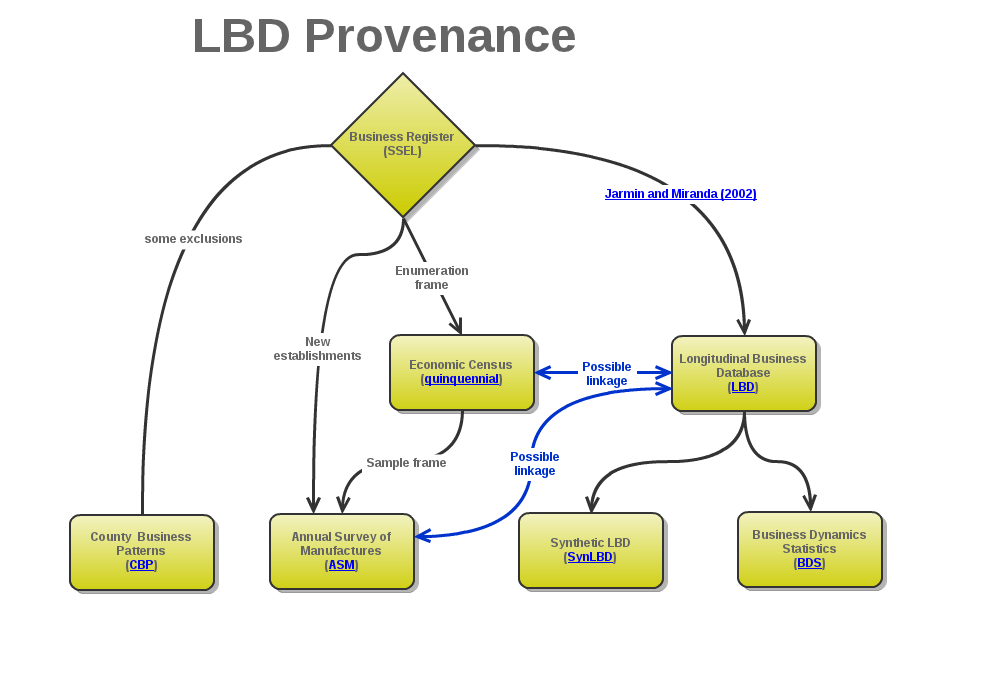
\includegraphics[width=\textwidth]{LBD_Provenance.png}
\end{frame}

\begin{frame}{Incorporating PROV (LBD)}
	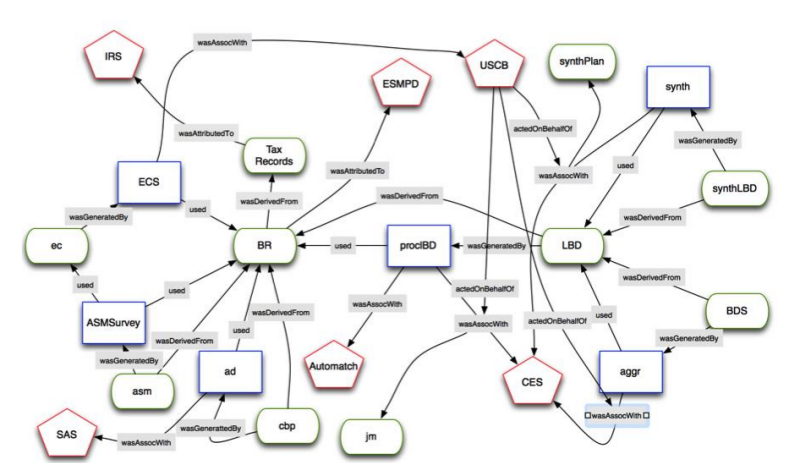
\includegraphics[width=0.9\textwidth]{LBD_Prov_simplified.png}
\end{frame}


\begin{frame}
	\frametitle{Provenance for research}
	\begin{block}{Sample research activity with full provenance}

	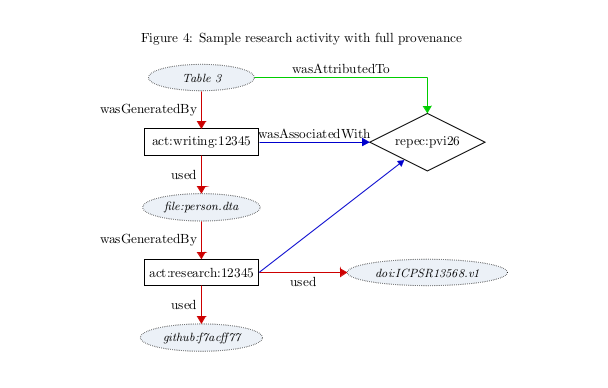
\includegraphics[scale=0.5]{tikz-authorship-example}
	\end{block}
\end{frame}


\begin{frame}
	\frametitle{Provenance for research}
	\begin{block}{Sample research activity with simple provenance}
		\centering
		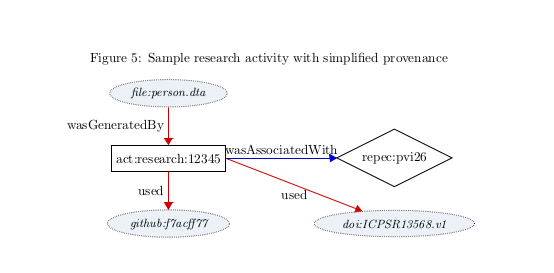
\includegraphics[scale=0.5]{tikz-authorship-example-simple}
	\end{block}
\end{frame}

\begin{frame}
\begin{beamercolorbox}[sep=8pt,center]{title}
	\usebeamerfont{title}Putting it together
\end{beamercolorbox}
\end{frame}


\begin{frame}
	\begin{beamercolorbox}[sep=8pt,center]{title}
		\usebeamerfont{title}Easy editing of all elements of data description
	\end{beamercolorbox}
\end{frame}

\begin{frame}
	\centering		
	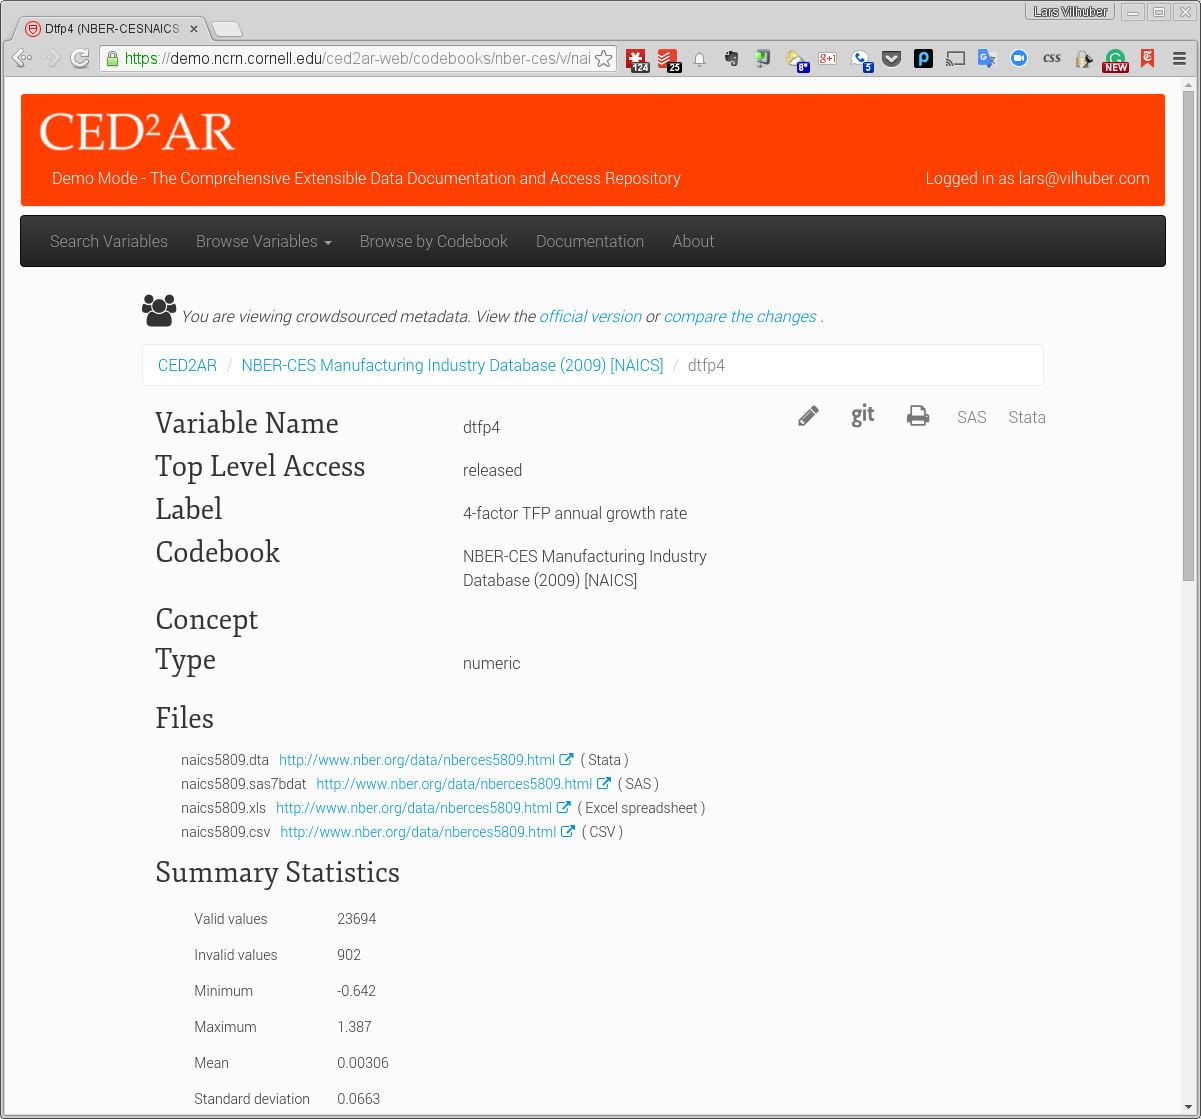
\includegraphics[height=\textheight]{Selection_133}
\end{frame}

\begin{frame}
	\centering		
	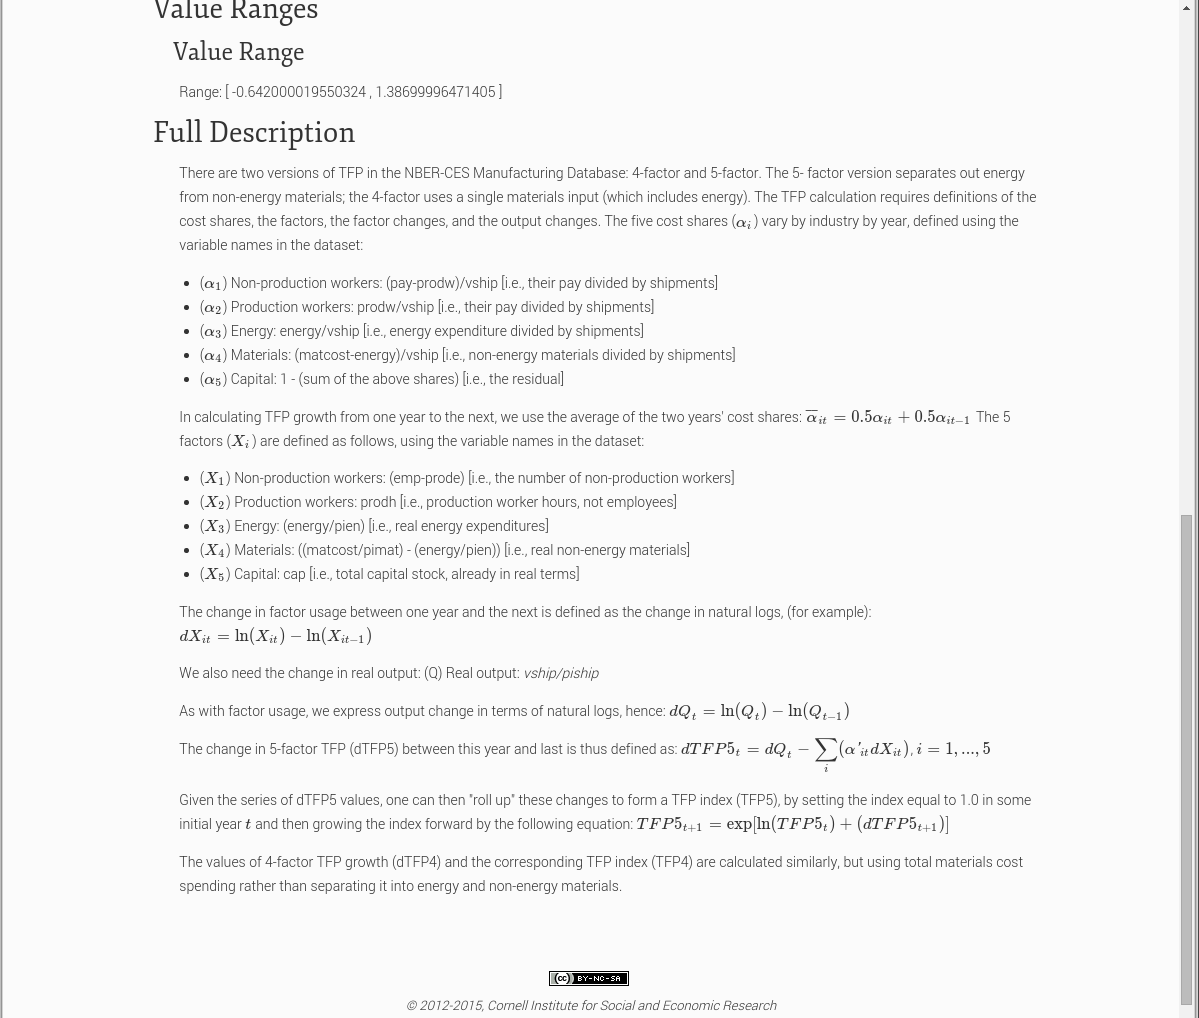
\includegraphics[height=\textheight]{Selection_134}
\end{frame}

\begin{frame}
	\centering		
	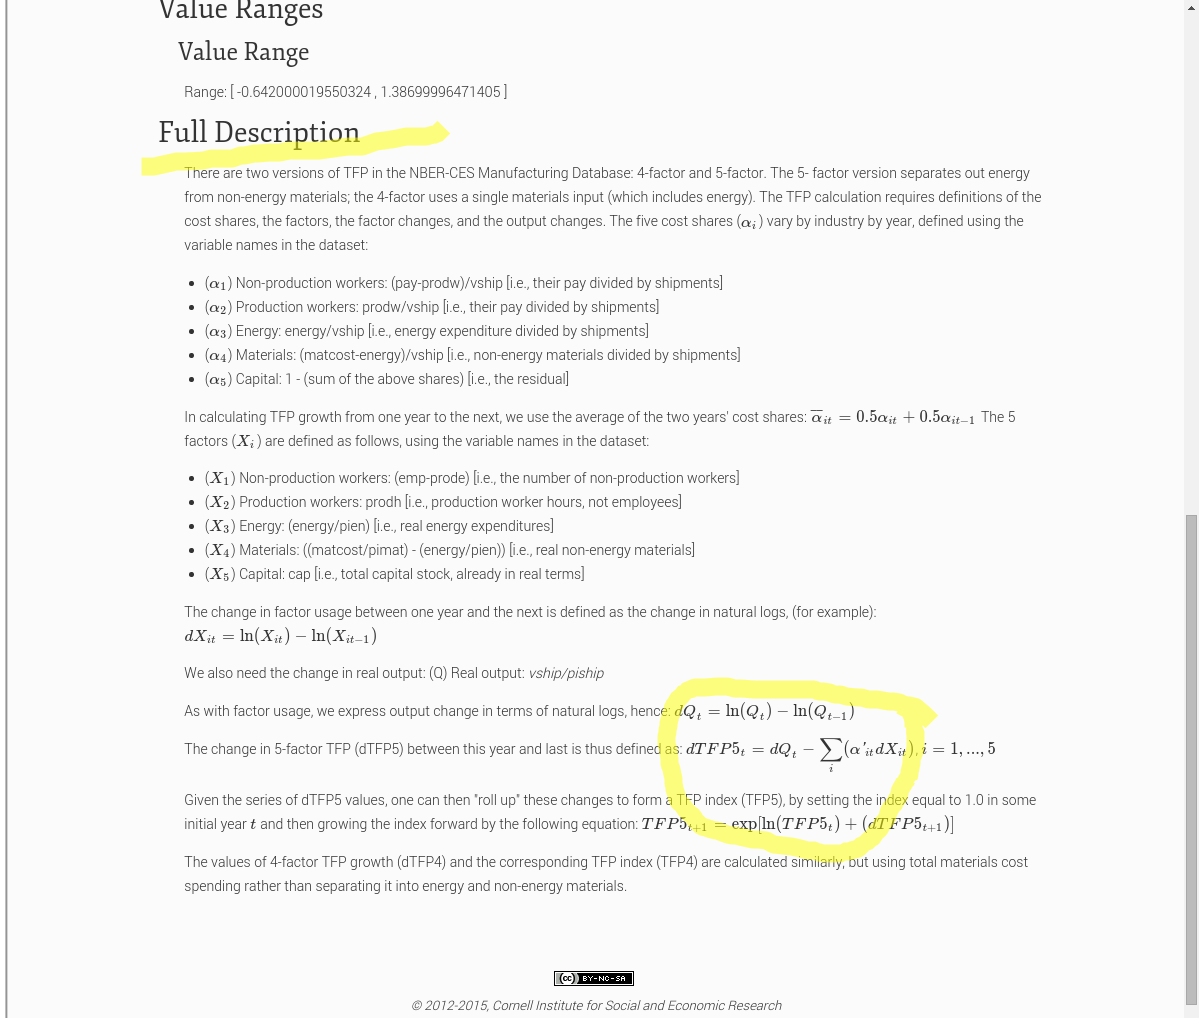
\includegraphics[height=\textheight]{Selection_134_hilite}
\end{frame}

\begin{frame}
	\frametitle{Lacking from other implementations}
	\begin{block}{... such as}
		\centering
		
\includegraphics[scale=0.5]{Selection_128}
		
	\end{block}
\end{frame}

\begin{frame}
	\begin{beamercolorbox}[sep=8pt,center]{title}
		\usebeamerfont{title}Editing of provenance
	\end{beamercolorbox}
\end{frame}


\begin{frame}
\centering		
		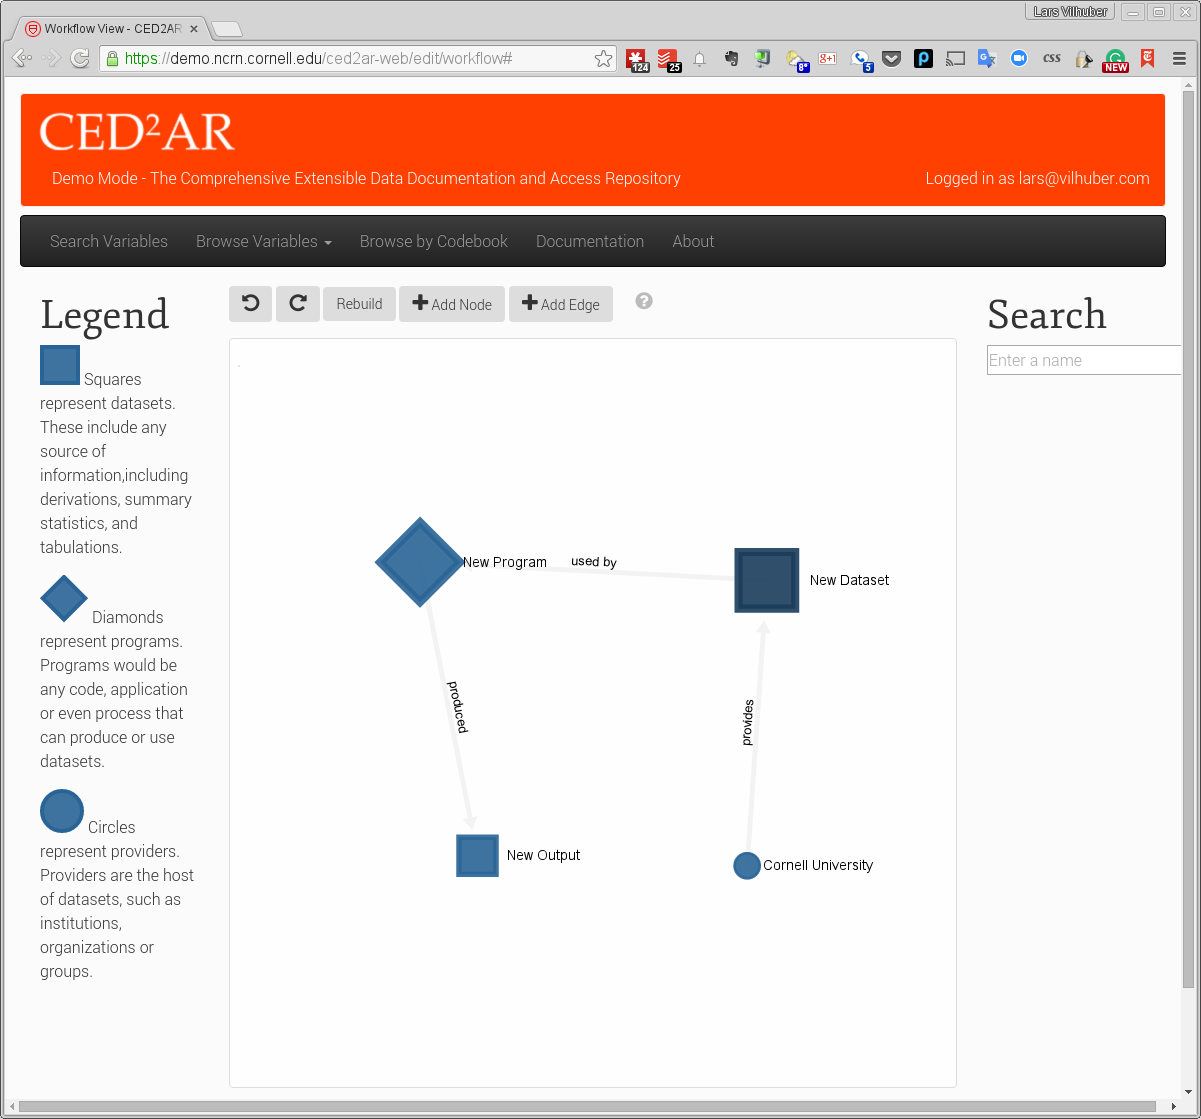
\includegraphics[height=\textheight]{Selection_132}
\end{frame}

\begin{frame}
	\frametitle{Possibilities}
	\begin{block}{Enhance journal or working paper archives}
		\begin{itemize}
			\item Capture the essential elements of programs, data, and how they are linked
		\end{itemize}
	\end{block}
	\begin{block}{Machine readable!}
	Because the metadata is structured, actionable data ensues
	\begin{itemize}
		\item Reproducible archives!
		\item Disclosure avoidance requests (Census RDC, German RDC require such documentation, but currently unstructured)
	\end{itemize}
	\end{block}
\end{frame}

\begin{frame}
	\frametitle{Additional elements}
	\begin{block}{Ex-post linking of articles and data}
		\centering

\includegraphics[scale=0.3]{Selection_129_hilight}
	\end{block}
\end{frame}

\begin{frame}
	\frametitle{Additional elements}
	\begin{block}{Ex-post linking of articles and data}
	\begin{itemize}
		\item Lacking from existing repositories of both data and bibliographies
		\item Exposure of data providers
		\item Sometimes manually (labor intensive) performed by data archives (e.g. ICPSR)
		\item Not currently done on RePEc
	\end{itemize}
	\end{block}
\end{frame}


\begin{frame}
	\frametitle{Crowd-sourcing data provenance}
	\begin{block}{Let other people contribute}
   \begin{tikzpicture}
   \node[draw=none,drop shadow={shadow scale=0.97,
   	top color=black,bottom color=gray,
   	shadow xshift=3pt,
   	shadow yshift=-2pt,
   	opacity=0.9}]
   at (1,1) {\fcolorbox{black}{white}{
\includegraphics[scale=0.3]{Selection_135}}}; \pause
   %
   \node[draw=none,drop shadow={shadow scale=0.95,
   	top color=black,bottom color=gray,
   	shadow xshift=3pt,
   	shadow yshift=-2pt,
   	opacity=0.9}]
   at (1,1) {\fcolorbox{black}{white}{
\includegraphics[scale=0.3]{Selection_136}}};
   \end{tikzpicture}		
	\end{block}
\end{frame}

\begin{frame}
	\frametitle{Crowd-sourcing data provenance}
	\begin{block}{Work in progress: on RePEc}
	\begin{itemize}
		\item Deploy a graphical interface that maps co-author networks, genealogy...
		\item ... and data provenance 
		\begin{itemize}
			\item incoming: what data did an article use? (LDI Replication workshop scaled up)
			\item outgoing: what data did an article create? (Better tracking of replication archives, or the National QWI example)
		\end{itemize}
		\item Users (or contributors!) can ``claim'' data, or if hosted on a data repository.
	\end{itemize}
	\end{block}
\end{frame}

\begin{frame}
	\frametitle{Other methods and efforts}
	\begin{block}{Similar linkage efforts}
		\begin{itemize}
			\item \href{http://www.rd-switchboard.org/}{RD-Switchboard}, based on \href{https://orcid.org/}{ORCID} IDs
			\item Direct DataCite/ORCID efforts
		\end{itemize}
	\end{block}
\end{frame}

\begin{frame}
\begin{beamercolorbox}[sep=8pt,center]{title}
	\usebeamerfont{title}... we've only barely started...
\end{beamercolorbox}
\end{frame}

%%% Local Variables:
%%% mode: latex
%%% End:

\ifpdf
\embedfile{Presentation-subdoc-replicability.tex}
\fi

%TCIDATA{Version=5.00.0.2570}
%TCIDATA{LaTeXparent=0,0,Presentation-CAFE-displacement-subdoc.tex}
% $Id: Presentation-subdoc-confidentiality.tex 1765 2015-11-11 12:50:51Z lv39 $
% $URL: https://forge.cornell.edu/svn/repos/lv39_papers/BigThinkPresentations/UQAM2015/Presentation/Presentation-subdoc-confidentiality.tex $
\section{Confidentiality}

\begin{frame}
	\frametitle{Limitations of restricted data access}
	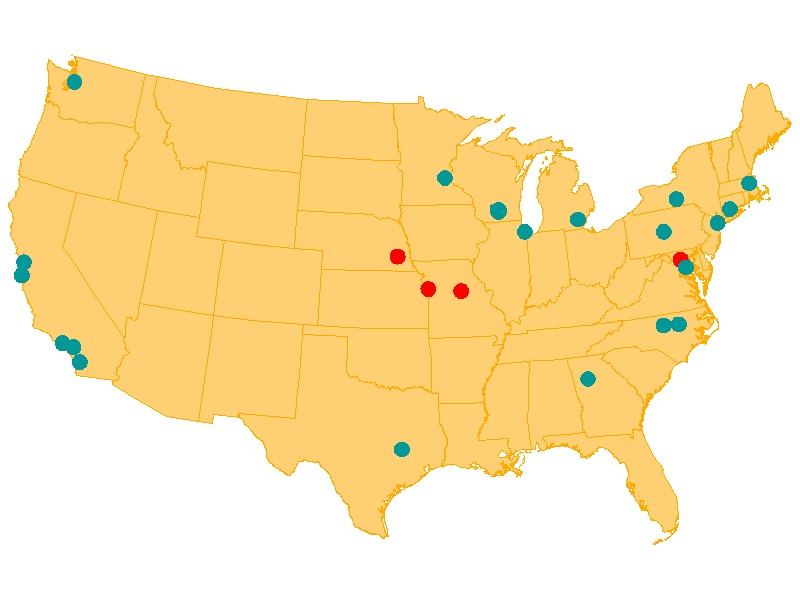
\includegraphics[width=\textwidth]{rdcmap_triad1c}
\end{frame}

\begin{frame}
	\frametitle{Limitations of restricted data access}
	\begin{block}{Users with access to (federal) confidential data in the US}
		There are {\large \textbf{21}} ({\small as of 2015-11-09}) Federal Research Data Centers (RDCs) in the US. There are approximately 300 researchers with access at any given time. (IRS: 12, BLS: 20?). There are currently {\large \textbf{6}} servers with total of 200+ CPUs available.
	\end{block}\pause
	\begin{block}{Users with access to public-use data}
		There are {\large \textbf{20-30} thousand} economists in the US. If they each have access to reasonably modern desktop, they have {\large \textbf{120k}} CPUs. Not counting compute clusters.
	\end{block}
\end{frame}

\begin{frame}
	\frametitle{Who wants to sit in this?}
	\begin{block}{UK efforts}
		\centering 
		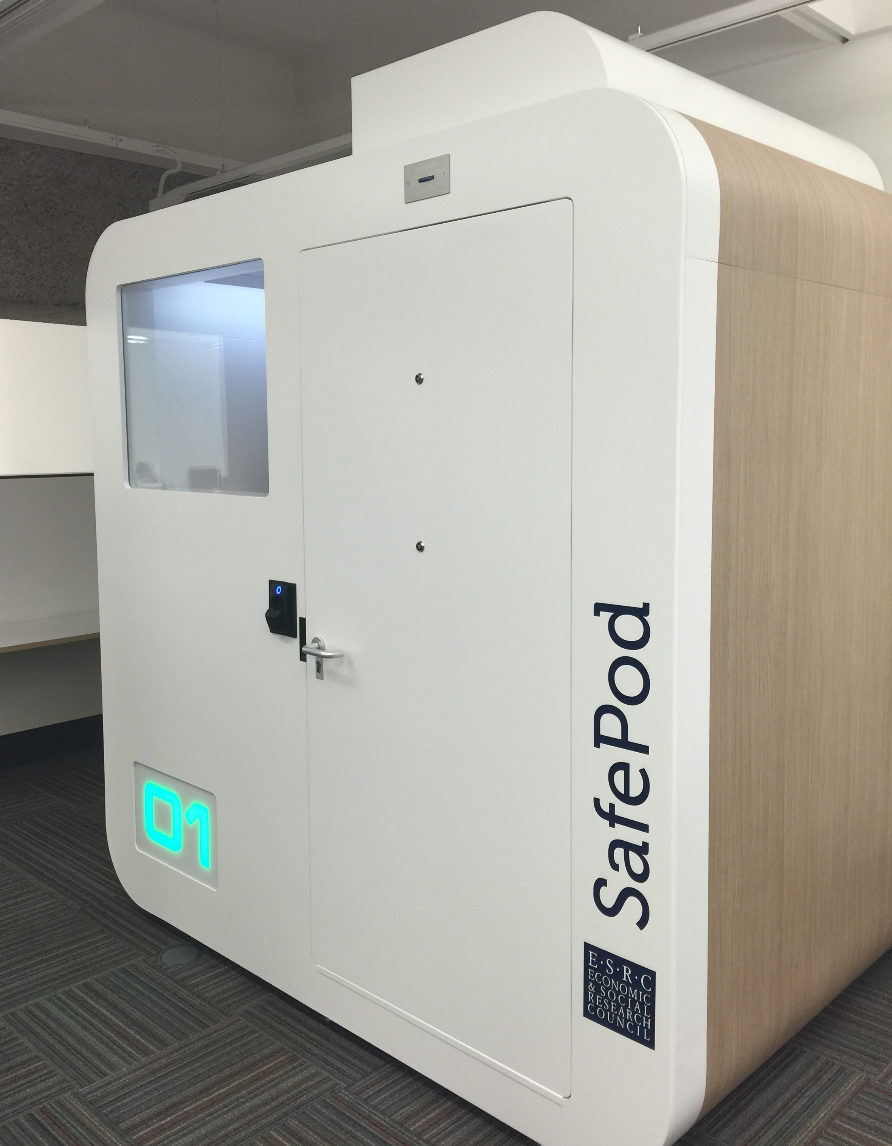
\includegraphics[height=0.8\textheight]{SafePODS}
	\end{block}
	
\end{frame}


\begin{frame}
	\frametitle{Who wants to sit in this?}
		\centering 
		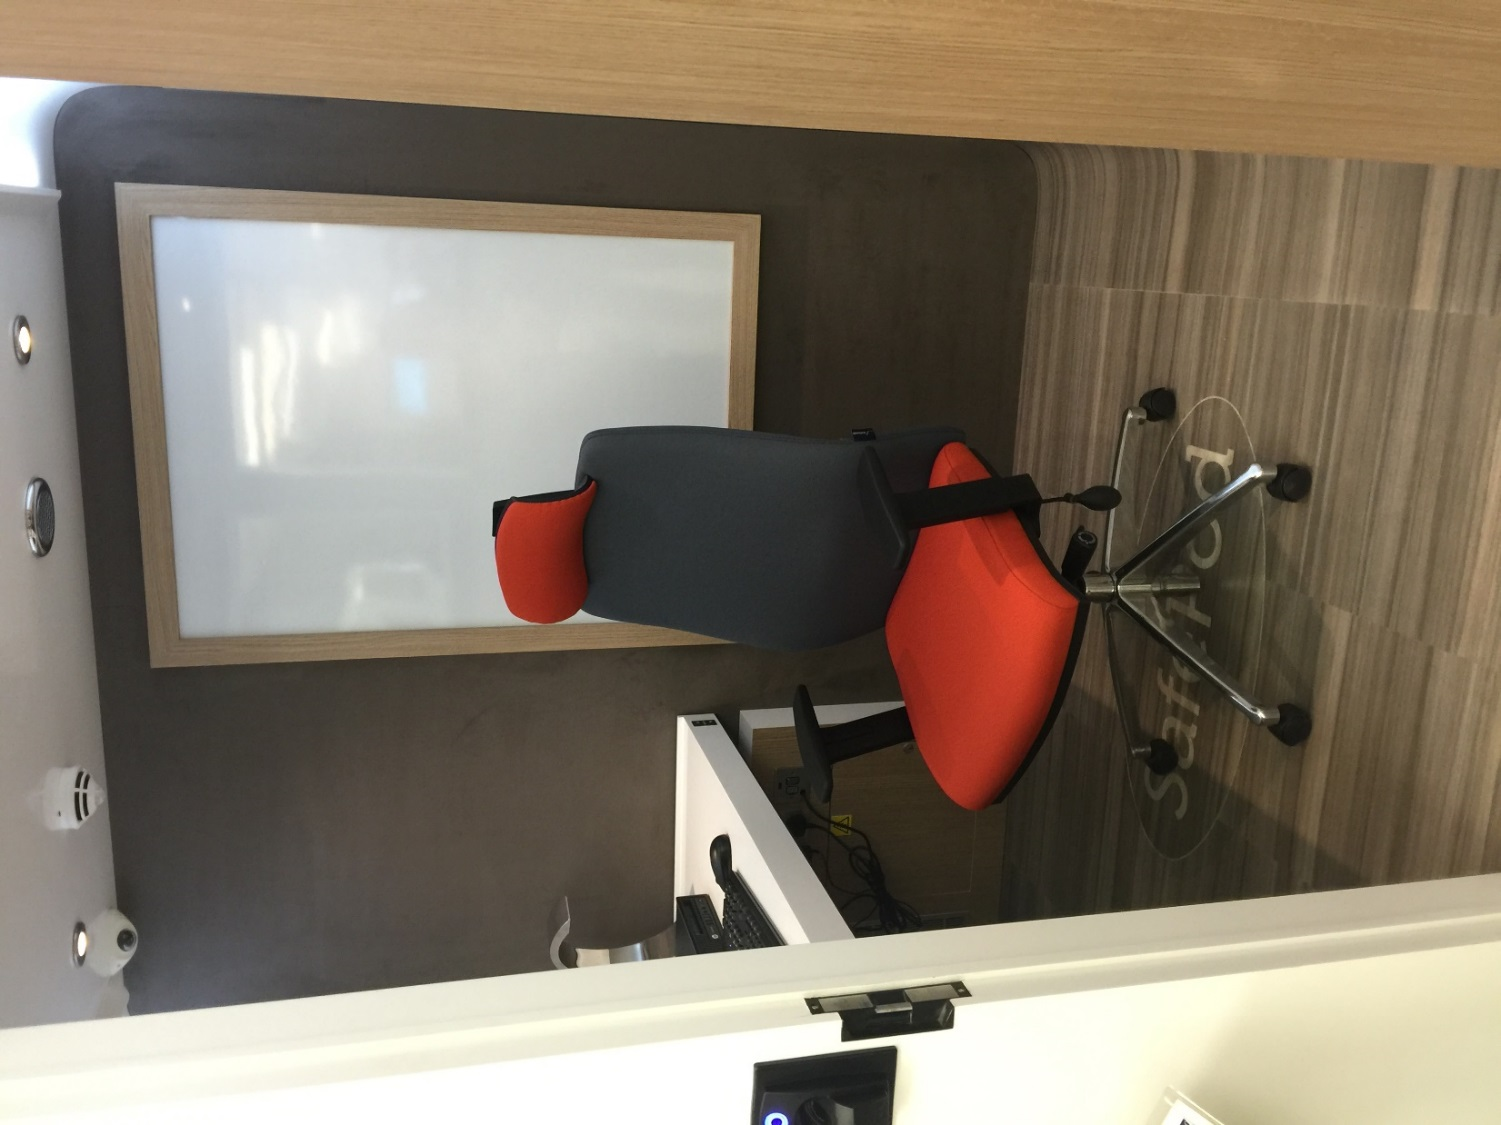
\includegraphics[height=0.6\textheight,angle=270]{SafePODS2}
		
	\tiny Src: \href{http://www1.unece.org/stat/platform/display/SDCWS15/}{Univ. Edinburgh -- Micro, remote, safe settings (safePODS) -- extending a safe setting network across a country}
\end{frame}



\begin{frame}
	\frametitle{Data liberation!}
{\Large Data curators trade off}
\begin{itemize}
	\item Providing detailed and accurate statistics 
	\item Protecting privacy and confidentiality 
\end{itemize}
\onslide<2>{\Large What is the optimal tradeoff, given the data have already been collected?}
\end{frame}

\begin{frame}
	\frametitle{Data curator strategies}
	\begin{block}{Limit access}
		\begin{itemize}
		    \item Let researchers run wild (with models)...
			\item ... and limit what can be removed (mostly adhoc)
			\item RDCs
			\item remote processing with delay and cost
		\end{itemize}
	\end{block}
	\begin{block}{Public-use files}
\begin{itemize}
	\item Disclosure limitation (aggregation, swapping, suppression, etc.)
\end{itemize}
	\end{block}
\end{frame}

\begin{frame}
	\frametitle{Some newer methods}
	\begin{block}{Multiplicative Noise Infusion}
		\begin{columns}
\begin{column}{0.7\textwidth}
	\footnotesize
\begin{equation*}
p\left( {\delta _{j}}\right) =\left\{ {{%
		\begin{array}{*{20}c} {\mbox{ }{\left( {b - \delta } \right)} \mathord{\left/ {\vphantom {{\left( {b - \delta } \right)} {\left( {b - a} \right)^2}}} \right. \kern-\nulldelimiterspace} {\left( {b - a} \right)^2},\;\delta \in \mbox{ 
				}\left[ {a,b} \right]} \\ {{\left( {b + \delta - 2} \right)} \mathord{\left/ {\vphantom {{\left( {b + \delta - 2} \right)} {\left( {b - a} \right)^2}}} \right. \kern-\nulldelimiterspace} {\left( {b - a} \right)^2},\;\delta \in \left[ {2 - b,2 - a} \right]\mbox{ }} \\ {0,\;\mbox{ otherwise }} \\ \end{array}%
				}}\right. 
\end{equation*}%
\begin{equation*}
				F\left( {\delta _{j}}\right) =\left\{ {{%
						\begin{array}{*{20}c} {\mbox{0},\;\delta < {2-b} } \\ {{\left[ {\left( {\delta + b - 2} \right)^2} \right]} \mathord{\left/ {\vphantom {{\left[ {\left( {\delta + b - 2} \right)^2} \right]} {\left[ {2\left( {b - a} \right)^2} \right]}}} \right. \kern-\nulldelimiterspace} {\left[ {2\left( {b - a} \right)^2} \right]},\;\delta \in \left[ {2 - b,2 - a} \right]\mbox{ }} \\ {\mbox{0.5}, \;\delta \in \mbox{ }\left( {2-a,a} \right)\mbox{ }} \\ {\mbox{0.5} + {\left[ {\left( {b - a} \right)^2 - \left( {b - \delta } \right)^2} \right]} \mathord{\left/ {\vphantom {{\left[ {\left( {b - a} \right)^2 - \left( {b - \delta } \right)^2} \right]} {\left[ {2\left( {b - a} \right)^2} \right]}}} \right. \kern-\nulldelimiterspace} {\left[ {2\left( {b - a} \right)^2} \right]},\;\delta \in \mbox{ }\left[ {a,b} \right]\mbox{ 
								}} \\ {\mbox{1}, \;\delta > {b} } \\ \end{array}}}\right. 
\end{equation*}%
\noindent where $a=1+{c}/{100}$ and $b=1+{d}/{100}$ are constants chosen
such that the true value is distorted by a minimum of $c$ percent and a
maximum of $d$ percent
\end{column}
\begin{column}{0.3\textwidth}
				
			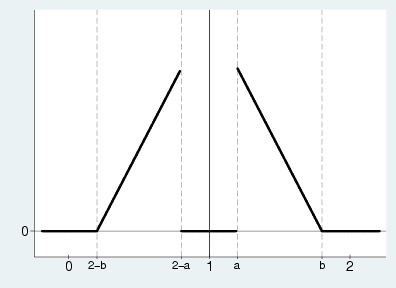
\includegraphics[width=0.9\textwidth]{fuzzfactors}
\vspace{0.5\textheight}
\end{column}	
\end{columns}
\end{block}
\end{frame}

\begin{frame}
	\frametitle{Applying noise infusion}
	\begin{block}{Quarterly Workforce Indicators}
Published value $X_{jt}^{\ast}$ computed from confidential value $X_{jt}$ as
\begin{equation}
X_{jt}^{\ast }=\delta _{j}X_{jt},  \label{eq:fuzz_totals}
\end{equation}%
	\end{block}
	See \href{https://ideas.repec.org/h/nbr/nberch/0485.html}{Abowd et al (2009)}
\end{frame}

\begin{frame}
	\frametitle{Synthetic data (Rubin, 1993; Little, 1993)}
	\begin{block}{Drawing from a posterior predictive distribution}
		\begin{itemize}
			\item[\ ] From data $\left ( X, Y ) \right )$, where $Y=\left ( Y_{obs}, Y_{nobs} \right )$
			\item[\ ] $I: i=0 \iff y \in Y_{nobs}$, 
			\item[\ ] construct PPD as $\left ( Y | X, Y_{obs}, I \right )$, and 
			\item[\ ] draw $Y^{\ast}$. 
			\item[\ ] Then release $\left ( X, Y^{\ast}_k \right )$ ($k$ partially synthetic data sets, typically $k>1$)
			\item[\ ] Similarity: $\left (X, (Y_{obs},Y_{nobs}^{\ast} ) \right )$ (multiply) imputed data
		\end{itemize}
	\end{block}
\end{frame}



\begin{frame}
	\frametitle{Examples of synthetic microdata}
	\begin{block}{SIPP Synthetic Beta}
		Survey of Income and Program Participation (SIPP) matched to administrative earnings, then synthesized
	\end{block}
	\begin{block}{Synthetic LBD (SynLBD)}
	   Longitudinal Business Database -- longitudinally linked establishment microdata -- synthesized
	\end{block}
\end{frame}

\begin{frame}
	\frametitle{Other uses of synthetic data}
	\begin{block}{American Community Survey tabulations}
		Group quarters
		\end{block}
		\begin{block}{LEHD Origin-Destination Employment Statistics (LODES)}
          Synthetic (differentially private) residence information combined with noise-protected establishment counts. (Machanavajjhala et al, 2008)
\end{block}
\end{frame}


\begin{frame}
	\begin{beamercolorbox}[sep=8pt,center]{title}
		\usebeamerfont{title} Key: analytic validity contingent on privacy protection
	\end{beamercolorbox}
	\centering \vspace{2cm}
How well does that work?
\end{frame}

\begin{frame}
	\frametitle{LODES}
	\centering
	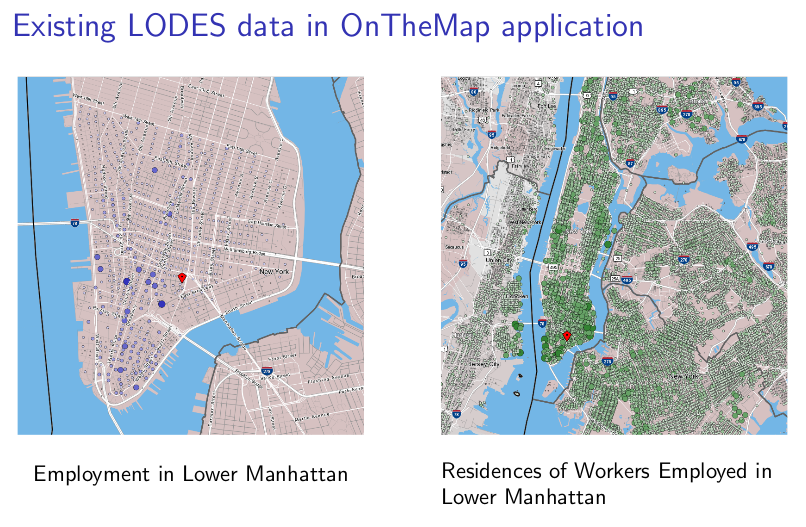
\includegraphics[width=0.9\textwidth]{sam-4}
\end{frame}


\begin{frame}
	\frametitle{Synthetic Data Server @ Cornell}
	\begin{block}{Open remote access}
		\begin{itemize}
			\item Users request account (no restrictions)
			\item Users run regression on synthetic data
			\item Users request validation against confidential data
		\end{itemize}
	\end{block}
\end{frame}

\begin{frame}
	\frametitle{Bertrand et al 2015}
	\begin{block}{From Bertrand et al (2015)}
		\centering
	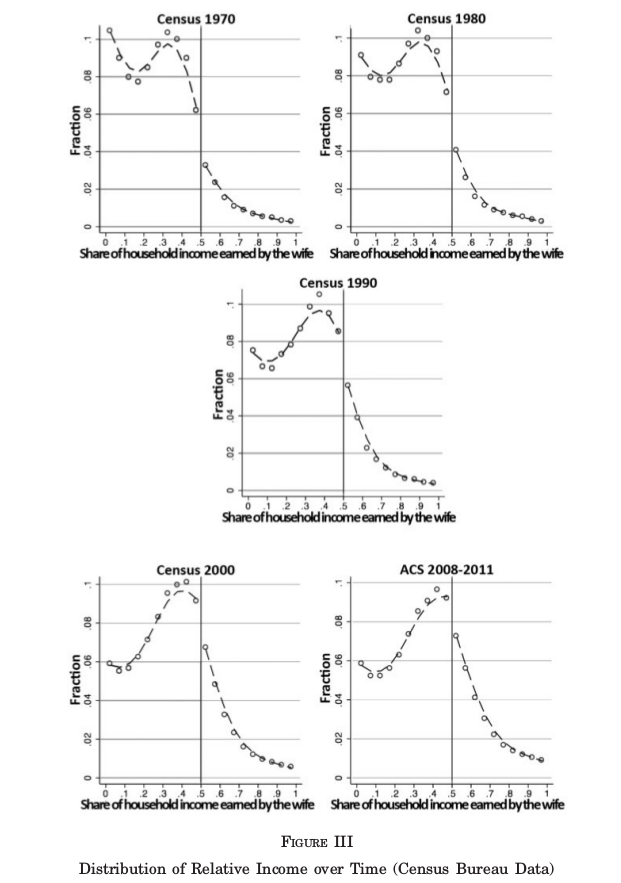
\includegraphics[width=0.5\textwidth]{Bertrand-QJE-2015-FigureIII}
\end{block}
\end{frame}



\begin{frame}
	\frametitle{Bertrand et al 2015}
	\centering
	{From Bertrand et al (2015), their Figure~I}
	\begin{tabular}{cc}
		(a) & (b)\\
		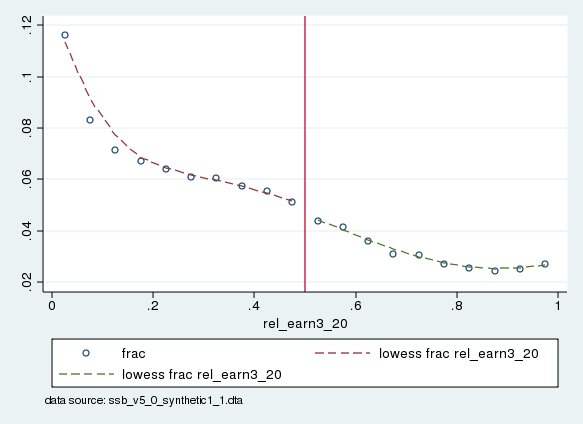
\includegraphics[width=0.4\textwidth]{jma_graph_rel_earn3_syn}&\pause
		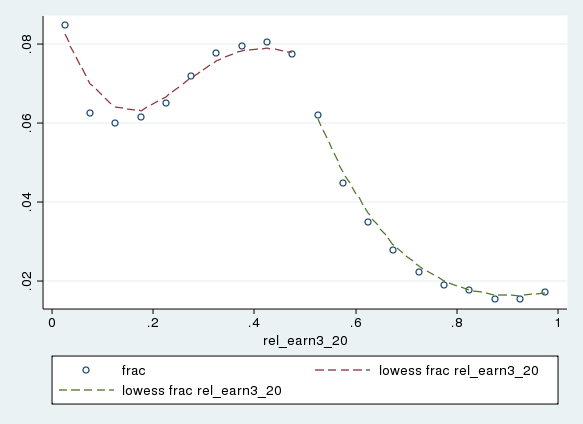
\includegraphics[width=0.4\textwidth]{jma_graph_rel_earn3}\\
	\end{tabular}
\end{frame}


\begin{frame}
	\frametitle{Synthetic data as a `blind commitment' device}
	\begin{block}{``Blind analysis: Hide results to seek the truth''}
		\href{http://www.nature.com/news/blind-analysis-hide-results-to-seek-the-truth-1.18510}{Nature, October 7, 2015}
``		\begin{quote}
			temporarily and judiciously removing data labels and altering data values to fight bias and error
		\end{quote}''
	\end{block}
	Synthetic data together with validation provides such a mechanism.
\end{frame}


\begin{frame}
	\frametitle{Bertrand et al 2015}
	\centering
	{From Bertrand et al (2015), their Figure~I}
\begin{columns}
	\begin{column}{0.5\textwidth}
		\centering
%	\begin{tabular}{p{.4\textwidth}p{.4\textwidth}}
%		(a) & (b)\\
		\only<1>{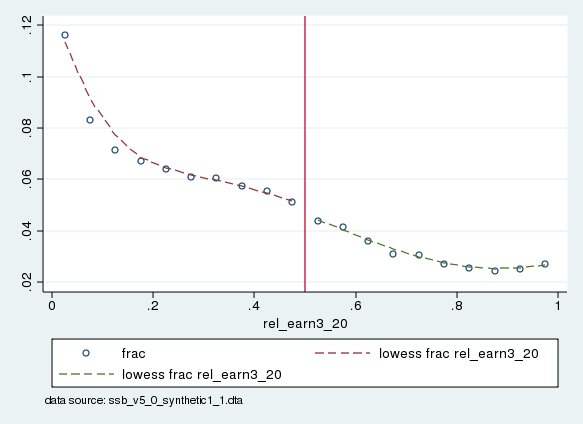
\includegraphics[width=0.95\textwidth]{jma_graph_rel_earn3_syn}}
	    \only<2>{Lifting of veil}
		\end{column}
%		&%\pause
\begin{column}{0.5\textwidth}
	\centering
		\only<2>{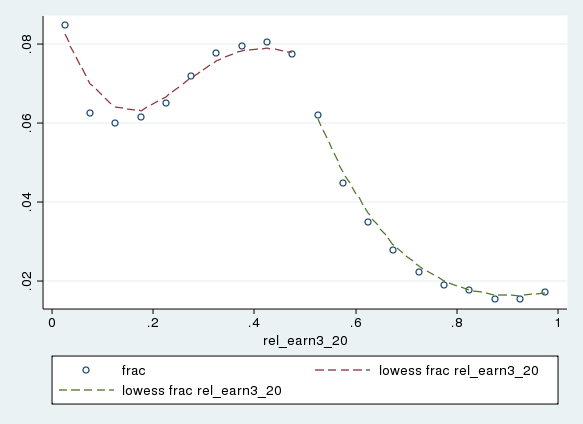
\includegraphics[width=0.95\textwidth]{jma_graph_rel_earn3}}
		\only<1>{ Blind model specification}\\

\end{column}	
%\end{tabular}
\end{columns}
\end{frame}


\begin{frame}
	\frametitle{Importance of feedback loop}
	\begin{block}{Account creation and events SDS}
		\centering
		
		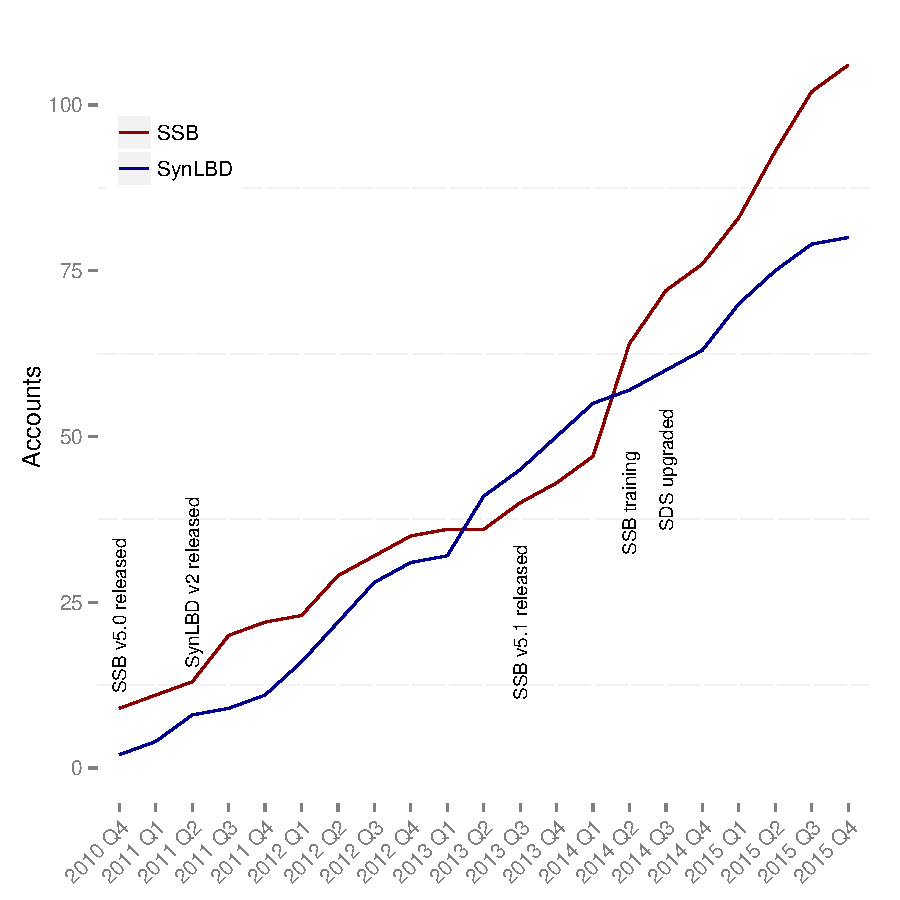
\includegraphics[width=0.6\textwidth]{report_on_SDS_2015_SOLE-accounts}
	\end{block}
\end{frame}

\begin{frame}
	\frametitle{More general validity results}
	Consider the overlap of confidence intervals $(L,U)$ for $\beta_{k,m}$ (estimated from the confidential data) and $(L^{*},U^{*})$ for $\beta_{k,m}^*$ (from the synthetic data).
	\begin{block}{Confidence interval overlap (Karr et al 2006)}
		\begin{itemize}
			\item[\ ]  Let $L^{over} = \max (L,L^{*} )$ 
			\item[\ ]  Let $U^{over} = \min (U,U^{*})$. 
			\item[\ ] Compute $J_{k,m}$ for parameter $k$ in model $m$. 
	\end{itemize}
Then the average overlap in confidence intervals 		
$$
J_{k,m}^{*} = \frac{1}{2} \left [ \frac{U^{over} - L^{over}}{U-L} + \frac{U^{over} - L^{over}}{U^*-L ^*}        \right ]
$$

We then average $J_{k,m}^{*}$ over all estimated models and parameters
\end{block}
\end{frame}


\begin{frame}
	\frametitle{Results from 3000 models and 14000 parameters}

\begin{table}[ht]
\caption{Confidence interval overlap $J_{k,m}^{*}$\label{tab:coverage}}
\centering
	\begin{tabular}{lrrrrr}
User&Request&  Mean&  75th & 90th & Max  \\
		   \hline
A    &1     & 0.160&  0.246 & 0.725& 0.889      \\%spec273
A    &2     & 0.101&  0     & 0.523& 0.924      \\%spec273
B%    &1     & 0.869&  1.000 & 1.000& 1.000      \\%spec444
C    &1     & 0.219&  0.509 & 0.725& 0.995      \\%spec527
	\end{tabular}
	
\end{table}
% Manually transcribed from email Oct 29 2015
	



\end{frame}

\begin{frame}
	\begin{beamercolorbox}[sep=8pt,center]{title}
		\usebeamerfont{title} Caution: large number of queries exhaust the ``privacy budget''
	\end{beamercolorbox}
\end{frame}
\newcommand{\M}{\mathcal{M}}
\begin{frame}[fragile]
	\frametitle{Protection against all possible queries}
	\begin{block}{Differential privacy}

					Let $\M$ be a randomized algorithm. Let $D$ and $D'$ be tables that differ in the presence of a single record (\textit{neighbors}). $\M$ satisfies $(\epsilon, \delta)$-differential privacy if for all $S \subseteq range(\M)$,
$$
			\log \frac{\Pr[\M(D) \in S]}{\Pr[\M(D') \in S] + \delta} \ \le \ \epsilon
$$

		$\delta$ allows for the ratio of probabilities to be unbounded with a small failure probability. To avoid algorithms that disclose individual records, $\delta$ should be set smaller than $1/n$. 
	\end{block}
\end{frame}


\begin{frame}
	\frametitle{Information content is limited}
	\begin{block}{Sequence of queries matters}
		\begin{itemize}
		    \item Order matters!
			\item Data custodian must decide which queries (=tables) to release first
			\item Then leave remaining privacy budget to researchers (?)
		\end{itemize}
	\end{block}
	\begin{block}{No free lunch}
         No information can be released without some privacy loss.
	\end{block}
\end{frame}


\begin{frame}
	\frametitle{Abowd and Schmutte (2014, 2015)}
\frametitle{Accuracy}
\begin{definition}[$(\protect\alpha ,\protect\beta )$-accuracy]
	\label{def:acc} A query release mechanism $M$ satisfies $(\alpha ,\beta )$%
	-accuracy for query sequence $\left\{ f_{1},f_{2},\ldots ,f_{k}\right\} \in
	\mathcal{F}^{k}$, $0<\alpha \leq 1$, and $0<\beta \leq 1$, if
	$$\min_{1\leq i\leq k}\left\{ \Pr \left[ |a_{i}-f_{i}(x)|\leq \alpha \right] \right\} \geq
	1-\beta. $$%
\end{definition}
		\end{frame}

\begin{frame}
	\frametitle{Abowd and Schmutte}
	\begin{block}{Model the demand for accuracy (social welfare function SWF)}
\centering
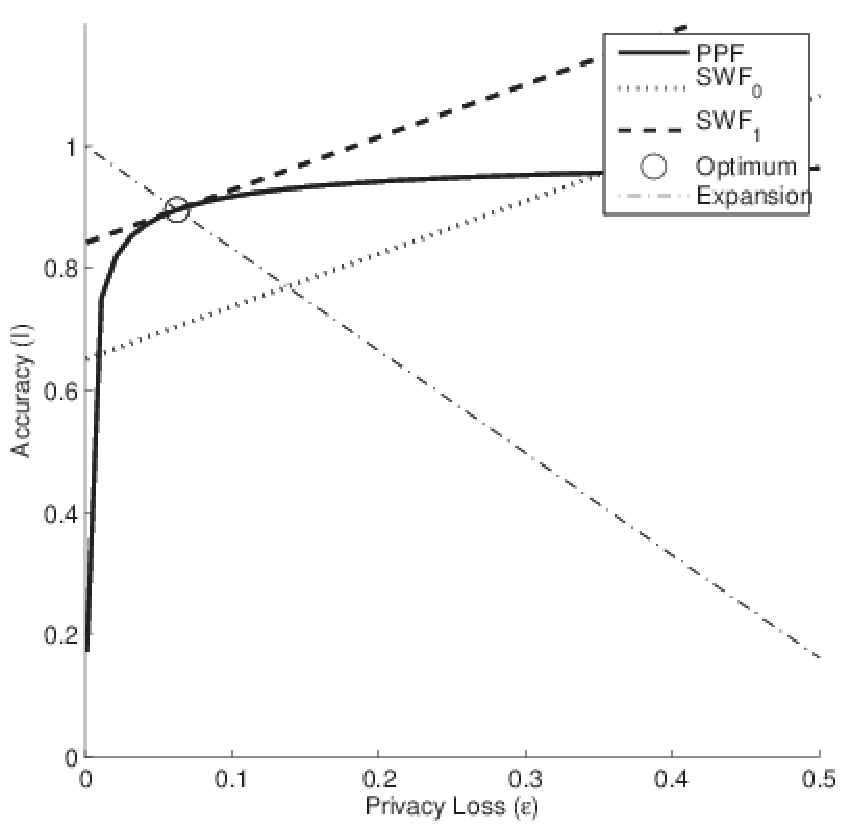
\includegraphics[width=0.6\textwidth]{plannersprob_health_complex}		
	\end{block}
\end{frame}
 \begin{frame}

 \frametitle{Technology for Anonymization}

 \textbf{Intuition:} Online Query Mechanism
 \begin{enumerate}
 	\item User sends query\vspace{.25in} 
 	\item Mechanism returns random output conditional on
 	\begin{itemize}
 		\item database
 		\item history\vspace{.25in} 
 	\end{itemize}
 	\item Use mechanisms that are provably \textit{differentially private}

 \end{enumerate}
 \end{frame}


\begin{frame}
	\frametitle{Relevancy to medical applications}
\begin{block}{Confidentiality and socio-medical data}
\begin{itemize}
	\item Restricted-access: e.g. \ac{HRS} biomarkers (same level of confidentiality as other more detailed data)
	\item Restricted remote access (remote data enclave): health insurance (``all-payer'') claims data (APCDs) [\ac{HCCI}]
	\item Trade-off: \ac{MIDUS} coarsens geography, but does not modify biomarkers
\end{itemize}

\end{block}

\end{frame}



\begin{frame}
	\frametitle{Relevancy to medical applications}\centering
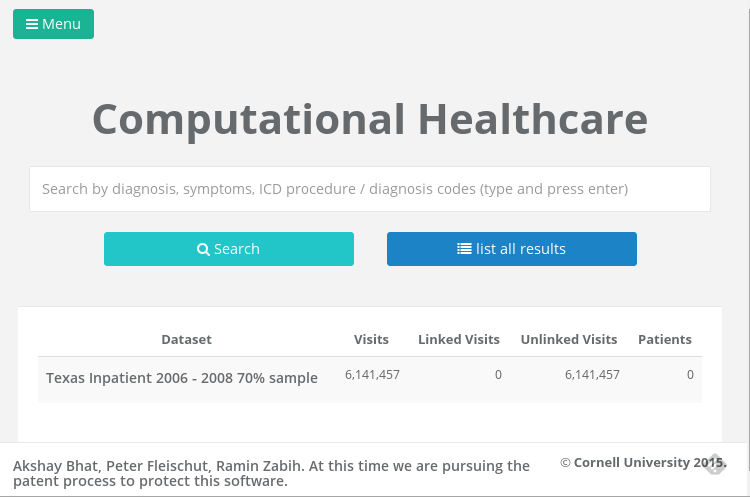
\includegraphics[width=0.8\textwidth]{Screenshot_system_20151002}
\end{frame}

\begin{frame}
	\frametitle{Relevancy to medical applications}\centering
	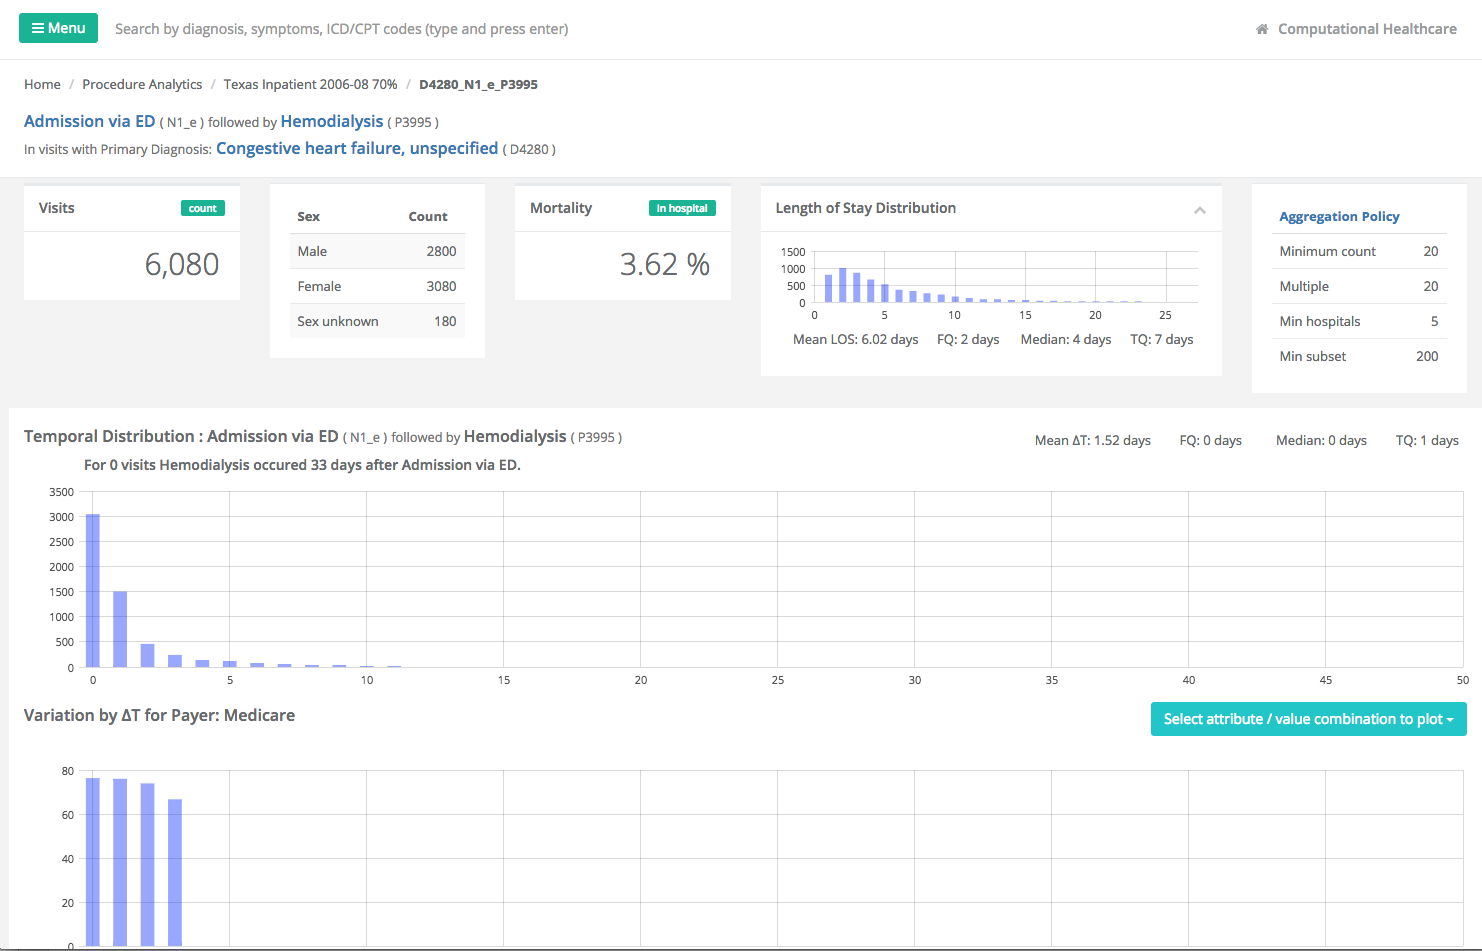
\includegraphics[width=0.8\textwidth]{Screenshot_system_20151003}
	\end{frame}

\begin{frame}
	\frametitle{Interactively exploring the technological frontier}
	\begin{block}{Active use is critical}
Provide users with an online query frontend that
interfaces directly with the confidential data, providing differentially private answers. This may still require
that all users be authorized users (TBD), and may be appropriate for certain research hospital settings.	The benefit would come from agency-signoff on the mechanisms, obviating the need for each user to be an authorized user.
\end{block}
\begin{block}{Exhaustion of information content}
Once the privacy budget is exhausted through the sequence of queries, any additional queries are rejected (yield a null set), because answering them is no longer possible without decreasing somebody's privacy beyond the allowed limit.
\end{block}
\end{frame}

\begin{frame}
	\frametitle{Silver lining}
	\begin{block}{How limiting the mechanism is...}
		Analyses that are provably dependent upon only the query set used to generate the current generation of
		the synthetic data are provably analytically valid with accuracy that is a function of the ($\alpha$,$\beta$)-accuracy used
		to generate the synthetic data.
	\end{block}
\end{frame}

%%% Local Variables:
%%% mode: latex
%%% End:

\ifpdf
\embedfile{Presentation-subdoc-confidentiality.tex}
\fi


\section{Conclusion}

\begin{frame}
	\frametitle{Tying it together}
	\begin{block}{Guiding light}
		Make data more accessible, by first-time users and by re-users.
	\end{block}
\end{frame}

\begin{frame}
	\frametitle{Provenance and synthetic data}
	\begin{block}{Reproducible analysis is key}
\begin{itemize}
	\item In order to simulate		Iterative Database Construction (IDC), we need to be able to re-run a suite of analysis.
	\item Structure imposed by \ac{SDS} is useful
	\item Actionable metadata is critical for scalability
\end{itemize}
	\end{block}
\end{frame}


\ifpdf
\embedfile{Presentation-subdoc-conclusion.tex}
\fi

%%TCIDATA{Version=5.00.0.2570}
%TCIDATA{LaTeXparent=0,0,Presentation-CAFE-displacement-subdoc.tex}
% $Id: Presentation-subdoc-synbds.tex 1764 2015-11-11 12:26:25Z lv39 $
% $URL: https://forge.cornell.edu/svn/repos/lv39_papers/BigThinkPresentations/UQAM2015/Presentation/Presentation-subdoc-synbds.tex $














\begin{frame}
\begin{block}{Business Dynamics}
"The U.S. economy is comprised of over 6 million establishments with paid employees. The population of these businesses is constantly churning -- some businesses grow, others decline and yet others close. New businesses are constantly replenishing this pool."[\href{https://www.census.gov/ces/dataproducts/bds/overview.html}{*}]
\end{block}
\begin{block}{Statistics at great detail on }
\begin{itemize}
\item job creation and destruction
\item establishment births and deaths
\item firm startups and shutdowns
\end{itemize}
by establishment and firm characteristics (age, size, location)
\end{block}
\end{frame}

%\begin{frame}{Business Dynamic Statistics}
%\begin{block}{Annual data series}
%\begin{itemize}
%\item Establishment - level business dynamics: by firm age and firm size
%\item Employment - job creation and destruction
%\item Job expansions and contractions
%\item Number of establishments
%\item Establishment openings and closings
%\item Number of startups and firm shutdowns   
%\end{itemize}
%\end{block}
%More info: 
%\href{http://www.census.gov/ces/dataproducts/bds/}{www.census.gov/ces/dataproducts/bds/}
%\end{frame}

\begin{frame}{Business Dynamic Statistics (BDS)}
\href{http://www.census.gov/ces/dataproducts/bds/}{www.census.gov/ces/dataproducts/bds/}
\begin{block}{Firm and Establishment Characteristics}
\begin{itemize}
\item Sector
\item Firm Size
\item Firm Age
\item Initial Firm Size
\item Geography (State, Metro/Non-metro, MSA)
\item Cross-tabulations by up to three of these characteristics
\end{itemize}
\end{block}
\begin{block}{Lots of detail}
\alert{Currently} 62 very detailed tables
\end{block}
\end{frame}

%\begin{frame}{Data for Business Statistics in the United States}
%\begin{block}{Provided by the US Census Bureau}
%\begin{itemize}
%\item County Business Patterns (CBP)
%\item Annual Survey of Manufactures (ASM)
%\item and over 100 separate additional surveys..
%\item Economic Census
%\item Business Dynamic Statistics (BDS)
%\item Quarterly Workforce Indicators (QWI)
%\end{itemize}
%\end{block}
%\pause
%\begin{block}{Provided by others}
%\begin{itemize}
%\item Quarterly Census of Employment and Wages (QCEW, by BLS)
%\item Compustat (S \& P), \acf{NETS}
%\end{itemize}
%\end{block}
%\end{frame}

\begin{frame}{Business Microdata at the Census Bureau}
\vfill
\Huge LBD-BDS complex
\end{frame}

\begin{frame}{Business Microdata at the Census Bureau}
\begin{center}
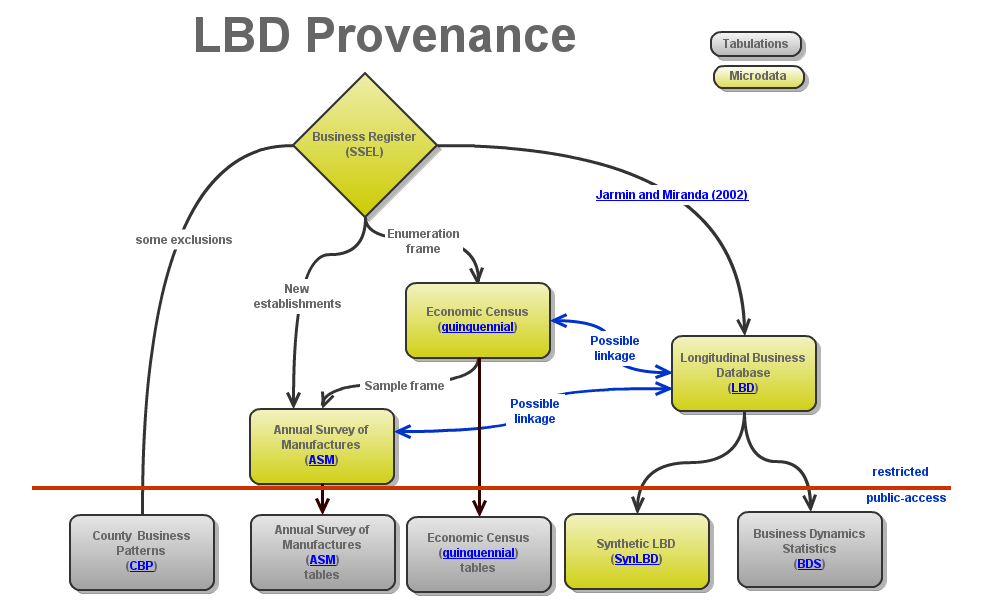
\includegraphics[height=0.8\textheight]{./LBD_Provenance_v2}
\end{center}
\end{frame}

\begin{frame}{Business Microdata at the Census Bureau}
\only<1>{
\begin{center}
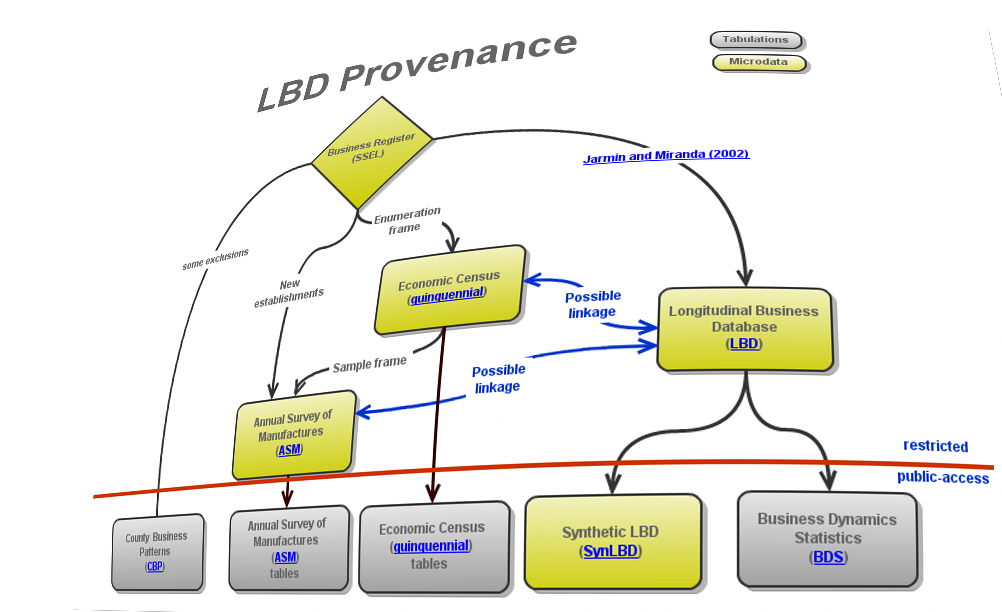
\includegraphics[height=0.8\textheight]{./LBD_Provenance_v2_tilted}
\end{center}}
\pause
\only<2| handout:0>{
\begin{center}
\includegraphics[height=0.8\textheight]{./LBD_Provenance_v2_tilted_hilite}
\end{center}}
\end{frame}





\begin{frame}{Disclosure avoidance in the BDS}
\begin{block}{P-percent rule with secondary suppressions}
\begin{itemize}[<+->]
\item Cells where the top 2 firms account for more than \emph{P} percent of the total value of the cell are flagged for suppression
\item \emph{P} value is not disclosed
\item Trivially: cells with fewer than 3 firms represented are always suppressed
\item Secondary suppressions: ``minimize the amount of information loss in a given table row or column''.
\end{itemize}
\end{block}
\end{frame}


\begin{frame}{Extent of suppression}
%\csvautotabular{programs/bds_e_suppressions_multi.csv}
\only<1| handout:0>{
\tiny
\begin{table}
\caption{Suppressions in establishment-level BDS\label{tab:bds_e}}
\centering
\begin{tabular}{|lc|r|rrr|}\hline%
               &                 &\bfseries Number &\multicolumn{3}{c|}{\bfseries Suppressions (\%)}\\
\cline{4-6}
\bfseries Type & \bfseries Level &\bfseries of     & & \multicolumn{2}{c|}{\bfseries Job creation}\\
                            &                              &\bfseries  cells& \bfseries Any  &\bfseries by entrants &\bfseries 
                            by continuers\\
\hline
\csvreader[head to column names,late after line=\\,late after last line=\\\hline]%
{../programs/bds_e_suppressions_multi.csv}{}%
{\typename & \level & \cells & \percentsup  & \jcbirths & \jcconts}%
\multicolumn{6}{p{0.8\textwidth}}{\tiny Note: Cells are year $x$ categories, where the 
number of categories varies by published table.}
\end{tabular}
\end{table}
}
\only<2>{
\begin{center}
\includegraphics[height=0.8\textheight]{./suppressions_estabs}
\end{center}
}
\end{frame}

\section[Solution]{Proposed solution}

\begin{frame}{Business Microdata at the Census Bureau}
\begin{center}
\includegraphics[height=0.8\textheight]{./LBD_Provenance_v2_tilted_hilite}
\end{center}
\end{frame}


\begin{frame}{Purpose of SynLBD}
\begin{block}{The SynLBD is }
\begin{itemize}[<+->]
\item synthetic establishment (and soon firm) microdata
\item derived from \alert{confidential} Longitudinal Business Database (LBD, 
\cite{MirandaJarmin2002})
\item designed to facilitate researcher access to establishment microdata (LBD) (see 
http://vrdc.cornell.edu/sds )
\item while preserving the confidentiality of establishment/business data. 
\item part of a larger strategy by the Census Bureau to provide \textit{better 
statistics on business dynamics} CNSTAT  \cite{CNSTATBusinessDynamics}
\end{itemize}
\end{block}
\end{frame}


\begin{frame}{Contents of (Syn)LBD}
\begin{block}{Data elements}
\begin{itemize}
\item  longitudinal establishment identifiers (created using probabilistic matching \cite{MirandaJarmin2002}) \onslide<2->{\alert{Masked}}
\item information on birth, death \onslide<2->{\alert{Synthesized}}
\item  employment and payroll over time \onslide<2->{\alert{Synthesized}}
\item location \onslide<2->{\alert{Suppressed}}
\item industry \onslide<2->{\alert{Released}}
\item firm  affiliation of  employer establishments \onslide<2->{\alert{$\rightarrow$ next version}}
\end{itemize}
\end{block}
\pause
\pause
\begin{block}{Complete description}
Kinney et al \cite{KinneyEtAl2011}
\end{block}
\tiny \hfill[\hyperref[sec:SynLBD_details]{more}]
\end{frame}

\begin{frame}
\begin{block}{Putting two and two together...}
\begin{itemize}[<+->]
\item[] 
V2.0 of SynLBD released by Census Bureau's Disclosure Review Board in 2011
\item[]
Let's combine public-use data to fill in suppressions

\end{itemize}
\end{block}
\end{frame}


%\begin{frame}{Combining synthetic and protected data}
%\begin{block}{Initially...}
%\begin{itemize}
%\item[...] explored as part of \href{http://www.myweb.ttu.edu/rgitting/}{Kaj Gitting}'s thesis 
%\cite{Gittings2009thesis}
%\item[...] expanded as part of our FCSM paper \cite{AbowdEtAl2012}
%\item[...] first stab at this in PSD 2014 presentation \cite{psd2014a}
%\end{itemize}
%\end{block}
%\end{frame}
%
%
%\begin{frame}{Ingredients for success}
%\begin{block}{Could it work for BDS?}
%\begin{itemize}
%\item BDS and SynLBD are ``siblings'', both derived from LBD
%\item SynLBD proven analytic validity
%\item SynLBD has authorized protection at microdata level - should persist to higher level 
%aggregations
%\item No need to republish previous BDS tabulations
%\end{itemize}
%\end{block}
%\end{frame}


\begin{frame}{Goal is two-fold}
\begin{block}{Retro-active utility}
A mechanism that can fill in existing suppressions.
\end{block}
\begin{block}{Improving disclosure avoidance going forward}
Evaluate future disclosure avoidance mechanisms:
\begin{itemize}
	\item Suppression
	\item This proposition
	\item Noise infusion (not here)
\end{itemize}
\end{block}
\end{frame}

\begin{frame}{Analytic validity}
\begin{center}
\only<1| handout:0>{
\includegraphics[height=0.8\textheight]{./CES-WP-11-04-page37}
}
\only<2>{
\includegraphics[width=\textwidth]{./CES-WP-11-04-page37-hilite}
}
\end{center}
\end{frame}

\begin{frame}{Analytic validity}
\begin{center}
\includegraphics[width=\textwidth]{./CES-WP-11-04-page39-hilite}
\end{center}
\end{frame}




\begin{frame}{Notation}

\begin{block}{Base variable}
Establishment employment $e_{jt}$. 
\end{block}
\begin{block}{Example}
\begin{eqnarray}
\label{eq:e_birth}
birth_{jt} &=& \left \lbrace 
\begin{array}{rl}
1 &\mbox{if}~~  e_{jt} > 0 ~~ \mbox{and}  ~~e_{jt-s} = 0 ~~\forall s\geq 1~~\\
0 &\mbox{otherwise}
\end{array} \right .
\end{eqnarray}
\begin{eqnarray}
\label{eq:e_birth2}
jcbirth_{jt} &=& \left \lbrace 
\begin{array}{rl}
e_{jt}-e_{jt-1} &\mbox{if}~~  e_{jt} > 0 ~~ \mbox{and}  ~~e_{jt-s} = 0 ~~\forall s\geq 1~~\\
0 &\mbox{otherwise}
\end{array} \right .
\end{eqnarray}
\end{block}
\end{frame}

\begin{frame}{Notation}
\begin{block}{Synthetic values}
Synthesized version of variable $x_{jt}$ is 
denoted $\tilde{x}_jt$. 
\end{block}
\begin{block}{Cells}
\begin{itemize}
\item[]
Collections of characteristics $k_t(j)$ (industry, geography, establishment or firm age and size)
\item[]  $j \in 
K_t^\prime$ describes the set of firms at time $t$ such that $k_t(j)=k^\prime$.  

\end{itemize}
\end{block}
\end{frame}

\begin{frame}{Notation}
\begin{block}{Aggregations}
Generically in capital letters:
\begin{equation}
\label{eq:national_e}
E_{\cdot t} = \sum_{j=1}^J e_{jt},
\end{equation}

Aggregations across establishments having characteristics $k^\prime$ at 
time $t$
\begin{equation}
\label{eq:sum_X}
X_{k^\prime t} =  \sum_{j \in K_t^\prime} x_{jt}
\end{equation}
\end{block}
\end{frame}

\begin{frame}{Suppression rules }
\begin{block}{Suppression rules}
for (aggregate) variable $X$ are captured by $I_{t}^X$, such that the 
releasable variable $X^{(0)}$  under the current regime can be described by

\begin{eqnarray}
\label{eq:supp_x}
X_{k^\prime t}^{(0)} &=& \left \lbrace 
\begin{array}{rl}
X_{k^\prime t} &\mbox{if}~~  I_{kt}^X = 1 \\
\mbox{missing} &\mbox{otherwise}
\end{array} \right .
\end{eqnarray}
\end{block}
\end{frame}



\subsection{Algorithm 1: Drop-in}
\begin{frame}[fragile]{Algorithm 1}

We can now express the simple ``drop-in'' algorithm, leading to the released variable $X^{(i)}$, 
as:
\begin{block}{BDS$^{(in)}$}
\begin{algorithm}
\begin{algorithmic}
\If {$I_{t}^X = 0$ }
        \State {$X_{k^\prime t}^{(i)} =\tilde{X}_{k^\prime t} $}
\Else
    \State {$X_{k^\prime t}^{(i)} = X_{k^\prime t} $}
\EndIf
\end{algorithmic}
\end{algorithm}
\end{block}
\end{frame}



\begin{frame}[fragile]{Weighted Algorithm 1}

\begin{block}{BDS$^{(i)}$}
\begin{algorithm}
%\caption{Weighted Drop-in}
{\bf Algorithm 1: Weighted Drop-in}
\hrule
\label{alg1}
\begin{algorithmic}
\State {$s^* = min_{s \in [0,n]} $ s.t. $I_{t-s}^X = 0$ }
\If { $n>0$ and $\exists s^*$ }
    \State {$X_{k^\prime t}^{(i)} =  \frac{s^*}{n} X_{k^\prime t}  
               + \left (1-\frac{s^*}{n} \right ) \tilde{X}_{k^\prime t} $}
\ElsIf { $n=0$ and $I_{t}^X = 0$}
    \State {$X_{k^\prime t}^{(i)} =  \tilde{X}_{k^\prime t} $}
\Else
        \State {$X_{k^\prime t}^{(i)} ={X}_{k^\prime t} $}               
\EndIf
\end{algorithmic}
\end{algorithm}
\end{block}
\end{frame}

%\begin{note}
%Thus, simply computing a ``SynBDS'', based on the \ac{SynLBD}, in parallel to the 
%computation 
%of the \ac{BDS} (based on the confidential \ac{LBD}), and replacing suppressed cells with their 
%fully synthetic counterparts, yields a dataset without missing observations. Variations can 
%encompass using the average of multiple implicates  as the replacement value. In 
%general, increasing the number of implicates will improve the analytic validity, but reduce the 
%protection provided by the synthesis process. 
%
%Because no time-consistency is imposed, this method can lead to seam biases or higher 
%intertemporal variance. We will return to this issue in Section~\ref{sec:analysis}. For later 
%reference, we denote the tabulations created by Algorithm~1 as \textbf{BDS$^{(i)}$}.
%\end{note}

\subsection{Algorithm 2: Weighted forward-longitudinal}

\begin{frame}{Algorithm 2}
\begin{block}{Similar idea, at microdata level}
Replace sensitive establishments with synthetic establishments.
\end{block}
\begin{block}{Smooth the replacement}
\begin{itemize}

\item per-establishment weight $w_{js} \in [0,1]$, applied to the observed data, that increases from 
$0$ in $t$ to $1$ in $t+n$, 
\item a per-establishment weight $\tilde{w}_{js}$, applied to the synthetic data, that decreases 
from $1$ in $t$ to $0$ in 
$t+n$, 
%\item thus ``blending in''  the real establishments, and ``blending out'' the synthetic 
%establishments.
	
\end{itemize}
\end{block}
\end{frame}

% Setting $w_{js} = 0, s \in [t,t+n-1]$ and $\tilde{w}_{js}=1, s \in [t,t+n-1]$ effectively 
%removes the real establishments from the tabulation, being completely  replaced by the synthetic 
%establishments.

\begin{frame}[fragile]{Algorithm 2}
	

	\begin{block}{BDS$^{(ii)}$}
\begin{algorithm}
%\caption{Forward-longitudinal}
{\bf Algorithm 2: Forward-longitudinal}
\hrule
\label{algorithm:2}
\begin{algorithmic}
\State {Compute: $X_{k^\prime t} = \sum_{j \in K_t^\prime} x_{jt}$}
\State{Compute: $I_{t}^X$}
\If {$I_{t}^X = 0$  }
   \State {// Suppression condition met for cell $k^\prime$}
    \State {Assign all $j \in K_t^\prime$ to $J_{k^\prime s}^-$ for $t \leq s \leq t+n$}
    \State {Assign all $j \in \tilde{K}_t^\prime$ to $J_{k^\prime t}^+$ for $t \leq s \leq t+n$}
\EndIf
\State { Compute: %
$$
X_{k^\prime t}^{(iiw)} = 
               \sum_{j \in \left \lbrace K_t^\prime \cap J_{k^\prime t}^+ \right \rbrace }
                               \tilde{w}_{jt} \tilde{x}_{jt} 
	          +
	          \sum_{j \in  K_t^\prime \wedge j \in J_{k^\prime t}^-  }
	                                  w_{jt}  {x}_{jt} 
	          +
	          \sum_{j \in  K_t^\prime \wedge j \notin J_{k^\prime t}^-  }
	                                         {x}_{jt} 
$$}

\end{algorithmic}
\end{algorithm}

	\end{block}
\end{frame}

\begin{frame}{Subtleties}

\begin{block}{Careful treatment of border cases}
\begin{itemize}
	\item Setting $n=0$ is similar to the "Drop-in" case, but margins add up
	\item Setting $w_{js} = 0$ for $s \in (t,t+n]$ simply replaces real establishments with synthetic establishments, no phase-in
	\item Synthetic establishments that are in cell $k^\prime$ in $t$ but are in cell $k^{\prime \prime}$ in $t+1$: should they receive $\tilde{w}_{jt+1}>0$?
\end{itemize}
\end{block}
\end{frame}



\section[Results]{Early results}


\begin{frame}{Analysis}
\begin{block}{Analysis}
\begin{itemize}[<+->]
\item We implemented Algorithm~1 and~2 for \ac{BDS} tabulations by \alert{establishment age 
and 
size} ({\tt bds\_e\_agesz}). 
\item Variations of $w$ and $n$
\item About 26\% of all cells have some suppression
\item Here: variable, ``Job Creation by establishment births'' ({\tt job\_creation\_births}) and 
``Job Creation by establishment continuers'' ({\tt job\_creation\_continuers}) 
\end{itemize}
\end{block}
\end{frame}

%\subsection{Protection}
%\begin{frame}{Protection}
%\begin{block}{Protection through synthesis}
%\begin{itemize}[<+->]
%\item Cells are filled in with data available to a wide audience (public-use)
%\item ....(but which typically cannot create tabulations)
%\item ....(future tables will contain variables which are not currently available on the synthetic 
%data file)
%\item Structurally: the synthetic data are ... fully synthetic (discussed in Kinney et al, 2011)
%\item Additional comparison: differences in each cell
%\end{itemize}
%\end{block}
%\end{frame}


\begin{frame}{Protection: From Kinney et al}
\begin{columns}
\begin{column}{0.6\textwidth}
\includegraphics[height=0.8\textheight]{CES-WP-11-04-page40-figure13}
\end{column}
\begin{column}{0.3\textwidth}
The comparison is for individual establishments, not within cells
\end{column}
\end{columns}
\end{frame}

\begin{frame}{Cell-wise comparison}
\begin{block}{Criteria for cell-wise comparison}
\begin{itemize}
\item Differences in count of establishment in a cell
\item Differences in values of cells
\end{itemize}
\end{block}

\end{frame}

\begin{frame}{Cell-wise comparison}
\includegraphics[width=0.9\textwidth]%
{results-synbds//graph_bds_release_vs_syn_pct_job_creation}

\end{frame}

\begin{frame}{Cell-wise comparison}
\includegraphics[width=0.9\textwidth]{results-synbds//graph_bds_release_vs_syn_pct_job_creation_births}

\end{frame}

\begin{frame}{Cell-wise comparison}
\includegraphics[width=0.9\textwidth]%
{results-synbds//graph_bds_release_vs_syn_pct_job_creation_continuers}

\end{frame}


\subsection{Analytic validity}

\begin{frame}{Analytic validity: time-series}
\begin{block}{Setup}
Estimate an AR(2) process for each of 
(confidential) $X_{k^\prime t}$, (synthetic) $X_{k^\prime t}^{(s)}$, $X_{k^\prime t}^{(i)}$, and 
$X_{k^\prime t}^{(ii)}$ (and their variants)
\end{block}
\begin{block}{Metrics}
\begin{itemize}
\item  number of missing time-series estimates/feasible regressions %(repeated suppressions in 
%$X_{k^\prime t}^{s}$ 
%may lead to time-series that are too short),
\item the number of significant coefficients for the first lag $\rho_1$ of the AR(2)
\item \emph{coverage}, the 
percentage of regressions where the true $\rho_1$ lies within the confidence band around the 
coefficient estimated from the comparison $\rho_1^{s}$ and $\rho_1^{(i)}$, 
\item interval overlap measure $J_k$ \cite{tas2006}
\end{itemize}
\end{block}
\end{frame}

\begin{frame}{$J_k$}
Consider the overlap of confidence intervals $(L,U)$ for $\rho_1$ (estimated from the 
confidential data) and $(L^{*},U^{*})$ for $\rho_1^*$. Let $L^{over} = \max (L,L^{*} )$ and 
$U^{over} = \min (U,U^{*})$. Then the average overlap in confidence intervals is

$$
J_k^{*} = \frac{1}{2} \left [ \frac{U^{over} - L^{over}}{U-L} + \frac{U^{over} - L^{over}}{U^*-L ^*}        \right ]
$$
We then average $J_k^{*}$ over all estimated AR(2) regressions.
\end{frame}

%\begin{frame}[fragile]{Analytic validity: Algorithm 1}
%\begin{center}
%
%
%%% Alternatively:
%\includegraphics[width=\textwidth]{table2}
%
%\end{center}
%\end{frame}


\begin{frame}[fragile]{Analytic validity: Percent missing}
	\begin{center}
		\footnotesize
		
		%% Alternatively:
		\begin{table}
\caption{Analytic validity: Feasibility of AR(2) regressions \label{tab:bds_e_pctmiss}}
\centering
%\begin{tabular}{|lc|r|rrr|}\hline%
\csvreader[tabular=|l|r|r|rrr|rrr|,table head=\hline 
	&Number 
	&\multicolumn{7}{c|}{Percent} 
\\
Variable 
	&feasible 
	& \multicolumn{7}{c|}{Infeasible}                
\\
    & $X_{k^\prime t}$ 
    & $X_{k^\prime t}^{(s)}$ 
    & $X_{k^\prime t}^{(0)}$ 
    & $X_{k^\prime t}^{(i)}$
    & $X_{k^\prime t}^{(in)}$
    & $X_{k^\prime t}^{(ii)}$
    & $X_{k^\prime t}^{(iiw)}$
    & $X_{k^\prime t}^{(iin)}$
    \\\hline,
	late after line=\\,late after last line=\\\hline]%
{../results/r_e_agesz_all_missing.csv}{Variable=\V,number=\colz,missing1=\cola,missing2=\colb,missing3=\colc,missing4=\cold,missing5=\cole,missing6=\colf,missing7=\colg}%
{\V &  \colz & \cola & \colb & \colc & \cold & \cole & \colf & \colg }%
\end{table}

		
	\end{center}
\end{frame}




\begin{frame}[fragile]{Analytic validity: Percent significant}
	\begin{center}
		\footnotesize
		
		%% Alternatively:
		\begin{table}
\caption{Analytic validity: AR(2) regressions with significant parameters\label{tab:bds_e_pctsign}}
\centering
%\begin{tabular}{|lc|r|rrr|}\hline%
\csvreader[tabular=|l|rr|rrr|rrr|,table head=\hline 
	& \multicolumn{8}{c|}{Percent} 
\\
Variable 
	& \multicolumn{8}{c|}{significant}
\\
    & $\rho_{1}$ 
    & $\rho_{1}^{(s)}$ 
    & $\rho_{1}^{(0)}$ 
    & $\rho_{1}^{(i)}$
    & $\rho_{1}^{(in)}$
    & $\rho_{1}^{(ii)}$
    & $\rho_{1}^{(iiw)}$
    & $\rho_{1}^{(iin)}$
    \\\hline,
	late after line=\\,late after last line=\\\hline]%
{../results/r_e_agesz_all_significant.csv}{Variable=\V,significantconf2=\colz,significant1=\cola,significant2=\colb,significant3=\colc,significant4=\cold,significant5=\cole,significant6=\colf,significant7=\colg}%
{\V &  \colz & \cola & \colb & \colc & \cold & \cole & \colf & \colg  }%
\end{table}

		
	\end{center}
\end{frame}


\begin{frame}[fragile]{Analytic validity: Coverage}
	\begin{center}
		\footnotesize
		
		%% Alternatively:
		\begin{table}
\caption{Analytic validity: AR(2) regressions: 
Coverage\label{tab:bds_e_coverage}}
\centering
%\begin{tabular}{|lc|r|rrr|}\hline%
\csvreader[tabular=|l|r|rrr|rrr|,table head=\hline 
	& \multicolumn{7}{c|}{} 
\\
Variable 
	& \multicolumn{7}{c|}{Coverage}
\\
    & $\rho_{1}^{(s)}$ 
    & $\rho_{1}^{(0)}$ 
    & $\rho_{1}^{(i)}$
    & $\rho_{1}^{(in)}$
    & $\rho_{1}^{(ii)}$
    & $\rho_{1}^{(iiw)}$
    & $\rho_{1}^{(iin)}$
    \\\hline,
	late after line=\\,late after last line=\\\hline]%
{../results/r_e_agesz_all_coverage.csv}{Variable=\V,coverage1=\cola,coverage2=\colb,coverage3=\colc,coverage4=\cold,coverage5=\cole,coverage6=\colf,coverage7=\colg}%
{\V &  \cola & \colb & \colc & \cold & \cole  & \colf & \colg }%
\end{table}

		
	\end{center}
\end{frame}

\begin{frame}[fragile]{Analytic validity: Overlap}
	\begin{center}
		\footnotesize
		
		%% Alternatively:
		\begin{table}
\caption{Analytic validity: AR(2) regressions: Interval 
overlap\label{tab:bds_e_jk}}
\centering
%\begin{tabular}{|lc|r|rrr|}\hline%
\csvreader[tabular=|l|r|rrr|rrr|,table head=\hline 
	& \multicolumn{7}{c|}{Interval} 
\\
Variable 
	& \multicolumn{7}{c|}{overlap}
\\
    & $J_k^{(s)}$ 
    & $J_k^{(0)}$ 
    & $J_k^{(i)}$
    & $J_k^{(in)}$
    & $J_k^{(ii)}$
    & $J_k^{(iiw)}$
    & $J_k^{(iin)}$
    \\\hline,
	late after line=\\,late after last line=\\\hline]%
{../results/r_e_agesz_all_Jk.csv}{Variable=\V,Jk1=\cola,Jk2=\colb,Jk3=\colc,Jk4=\cold,Jk5=\cole,Jk6=\colf,Jk7=\colg}%
{\V &  \cola & \colb & \colc & \cold & \cole & \colf & \colg }%
\end{table}

		
	\end{center}
\end{frame}









\section{Conclusion}

\begin{frame}{Open issues}
\begin{block}{Unexplored issues}
\begin{itemize}[<+->]
\item SynLBD is synthesized independently within industry
\item Geography is not synthesized, not considered within synthesis process (and not released) 
- unclear how geography subtabulations will fare, what the disclosure avoidance implications are
\item Firm-level characteristics go into a bit more detail, and require availability of SynLBD v3
\item Time consistency of the series
\item Comparison to alternative ``outside-the-firewall'' imputation mechanisms 
(\cite{HolanEtAl2010,BradleyEtAl2014})
\end{itemize}
\end{block}
\end{frame}


\begin{frame}{Conclusion}
\begin{block}{Early in the process}
\begin{itemize}
\item Desirable a-priori properties (use of public-use data to fill in blanks)
\item May not work for other variables
\item Assumes suppression as primary disclosure avoidance mechanism...
\end{itemize}\end{block}
\end{frame}

% trick to stop counting slides
\newcounter{finalframe}
\setcounter{finalframe}{\value{framenumber}}
% Backup frames
\setcounter{framenumber}{\value{finalframe}}


\begin{frame}
Thank you
\end{frame}


%\begin{frame}[fragile]
%
%\tiny\vspace{0.8\textheight}\vfill 
%\begin{verbatim}
%$Id: Presentation-subdoc-synbds.tex 1764 2015-11-11 12:26:25Z lv39 $
%\end{verbatim}
%\end{frame}



\begin{frame}[fragile]
\begin{center}
More info: 
\begin{itemize}
\item For information on the SynLBD, see 
\href{http://www2.vrdc.cornell.edu/news/data/lbd-synthetic-data/}{goo.gl/eyrv7w}
\item Access through the Synthetic Data Server, 
\href{http://www.vrdc.cornell.edu/sds/}{www.vrdc.cornell.edu/sds/} 
\end{itemize}

\end{center}
\tiny\vspace{0.8\textheight}\vfill 
\begin{verbatim}
$Id: Presentation-subdoc-synbds.tex 1764 2015-11-11 12:26:25Z lv39 $
\end{verbatim}
\end{frame}

%%% Local Variables:
%%% mode: latex
%%% End:

\ifpdf
\embedfile{Presentation-subdoc-synbds.tex}
\fi


{
	\usebackgroundtemplate{\includegraphics[width=\paperwidth]{2015_0795_015_select.jpg}}
	\frame{Merci}
}

\appendix
\part<presentation>{Appendix}

% $Id: Presentation-appendix.tex 1764 2015-11-11 12:26:25Z lv39 $ 
% $URL: https://forge.cornell.edu/svn/repos/lv39_papers/BigThinkPresentations/UQAM2015/Presentation/Presentation-appendix.tex $ 

\section{Extra slides}


%\begin{frame}
%\frametitle{Bibliography}
%\tiny
%\bibliography{../abbrev,../paper}
%\bibliographystyle{IEEEtranS}
%\end{frame}

\subsection*{Acronyms}
\begin{frame}{Acronyms}

%TCIDATA{Version=5.00.0.2570}
%TCIDATA{LaTeXparent=0,0,sw-edit.tex}

% $Id: acronyms.tex 1764 2015-11-11 12:26:25Z lv39 $
% $URL: https://forge.cornell.edu/svn/repos/lv39_papers/BigThinkPresentations/UQAM2015/Presentation/acronyms.tex $
%
% Define acronyms to be used in the text here. See
% http://www.mackichan.com/index.html?techtalk/456.htm~mainFrame for usage in
% Scientific workplace context

\begin{acronym}
% head -11 $(find . -name acronyms.tex -exec ls -l --full-time {} \; | sort -k 6 | tail -1 | awk ' { print $9 } ')  > /ramdisk/acronyms.tex
%cat $(find . -name acronyms.tex -exec ls -l --full-time {} \; | sort -k 6 | awk ' { print $9 } ') | sort | uniq > /ramdisk/acronyms.tex

\acro{ACS}{American Community Survey}
\acro{ACS-POW}{American Community Survey Place of Work file}
\acro{ACS-PUMS}{American Community Survey Public Use Microdata Sample}
\acro{AEA}{American Economic Association}
\acro{AHEAD}{Study of Assets and Health Dynamics Amongst the Oldest Old}
\acro{AHRQ}{Agency for Healthcare Research and Quality}
\acro{AHS}{American Housing Survey}
\acro{ASCII}{American Standard Code for Information  Interchange} %, typically used to denote raw text files in PC or Unix environments
\acro{ASM}{Annual Survey of Manufacturers}
\acro{BB}{Bayesian bootstrap}
\acro{BCC}{Bowie Computer Center}
\acro{BDS}{Business Dynamics Statistics}
\acro{BED}{Business Employment Dynamics}
\acro{BES}{Business Expenditure Survey}
\acro{BIC}{Bayes Information Criterion}
\acro{BLS}{Bureau of Labor Statistics}
\acro{BMF}{Block Map File}
\acro{BRB}{Business Register Bridge}
\acro{BRB}{LEHD Business Register Bridge}
\acro{BR}{Business Register}
\acro{BR}{Business Register\acroextra{, formerly known as the SSEL}}
\acro{CAC}{Cornell Center for Advanced Computing}
\acro{CBO}{Congressional Budget Office}
\acro{CBP}{County Business Patterns}
\acro{CBSA}{Core Based Statistical Area}
\acro{CBSA}{Core-Based Statistical Area}
\acro{CER}{Covered Earnings Records}
\acro{CES}{Center for Economic Studies}
\acro{CEW}{Covered Employment and Wages}%. Employment statistics program run by BLS in  conjunction with all states, also known as ES-202. Generally, when used  in this document, refers to public-use tabulations from the CEW, as  opposed to the confidential microdata received directly from the states.
\acro{CFN}{Census File Number}
\acro{CIA}{Central Intelligence Agency}
\acro{CISER}{Cornell Institute for Social and Economic Research}
\acro{CIT}{Cornell Information Technologies}
\acro{CM}{Census of Manufactures}
\acro{CNSS}{Cornell National Social Survey}
\acro{CODA}{Children of the Depression Age}
\acro{Code1}{Code 1\acroextra{, geocoding software from Group 1, now owned by Pitney Bowes}}
\acro{COLA}{cost of living allowance}
\acro{CPI}{Consumer Price Index}
\acro{CPI-U}{Consumer Price Index (All Urban Consumers)}
\acro{CPR}{Composite Person Record}
\acro{CPS}{Current Population Survey}
\acro{CRADC}{Cornell Restricted Access Data Center}
\acro{CRAN}{the Comprehensive R Archive Network\acroextra{, accessible at
\url{http://cran.r-project.org/} and natively within R}}
\acro{CSV}{Comma-separated values}
\acro{CTC}{Cornell Theory Center}
\acro{CTPP}{Census Transportation Planning Package}
\acro{DCC}{Data Confidentiality Committee}
\acro{DC}{Decennial Census}
\acro{DDI}{Data Documentation Initiative\acroextra{, see \href{http://www.ddialliance.org/}{http://www.ddialliance.org/}}}
\acrodef{err}{excess reallocation rate}
\acrodef{jcr}{job creation rate}
\acrodef{jdr}{job destruction rate}
\acrodef{jrr}{job reallocation rate}
\acrodef{wrr}{worker reallocation rate}
\acro{DER}{Detailed Earnings Record}
\acro{DHS}{Department of Homeland Security}
\acro{DMZ}{Demilitarized Zone}
\acro{DOI}{Digital Object Identifier}
\acro{DRB}{Disclosure Review Board}
\acro{DWS}{Displaced Worker Supplement}
\acro{ECF}{Employer Characteristics  File}
\acro{EHF}{Employment History Files}
\acro{EHRI}{Enterprise Human Resources Integration}
\acro{EIN}{\acroextra{(federal) }Employer Identification Number}
\acro{ERR}{Excess Reallocation Rate}
\acro{ES-202}{ES-202\acroextra{. An older name for the \ac{QCEW} program}}
\acro{FBI}{Federal Bureau of Investigation}
\acro{fCOI}{financial Conflict of Interest}
\acro{FCSM}{Federal Committee on Statistical Methodology}
\acro{FDIC}{Federal Deposit Insurance Corporation}
\acro{FEMA}{Federal Emergency Management Agency}
\acro{FHFA}{Federal Housing Finance Agency}
\acro{FIPS}{Federal information processing standards codes\acroextra{\ issued     by \ac{NIST}}}
\acro{FOIA}{Freedom of Information Act}
\acro{FSRDC}{Federal Statistical Research Data Center}
\acro{FTI}{Federal Tax Information}
\acro{GAL}{Geocoded Address List}
\acro{GAO}{Government Accountability Office}
\acro{GIS}{Geographic Information System}
\acro{GRF-C}{Geographic Reference File-Codes}
\acro{GRF}{Geographic Reference File}
\acro{GSA}{General Services Administration}
\acro{GSS}{General Social Survey}
\acro{HCCI}{Health Care Cost  Institute}
\acro{HCUP}{Healthcare Cost and Utilization Project}
\acro{HCEF}{100 Percent Census Edited File}
\acro{HDF}{100 Percent Detail File}
\acro{HHS}{\acroextra{Department of\ }Health and Human Services}
\acro{HIPAA}{Health Insurance Portability and Accountability Act}
\acro{HPI}{\ac{OFHEO} House Price Index}
\acro{HRS}{Health and Retirement Study}
\acro{ICF}{Individual Characteristics File}
\acro{ICPSR}{Inter-university Consortium for Political and Social Research}
\acro{IDC}{Iterative Database Construction}
\acro{IDSC}{International Data Service Center}
\acro{ILR}{Cornell School of Industrial and Labor Relations}
\acro{IPUMS}{Integrated Public Use Microdata Series}
\acro{IRB}{Institutional Review Board}
\acro{IRS}{Internal Revenue Service}
\acro{ISBN}{International Standard Book Number}
\acro{ISR}{Institute for Social Research}
\acro{ISSN}{International Standard Serial Number}
\acro{IZA}{Institute for the Study of Labor}
\acro{HRS}{Health and Retirement Survey}
\acro{JCR}{Job Creation Rate}
\acro{JDR}{Job Destruction Rate}
\acro{JHF}{Job History File}
\acro{JOLTS}{Job Openings and Labor Turnover Survey}
\acro{JRR}{Job Reallocation Rate}
\acro{JSM}{Joint Statistical Meetings}
\acro{KDE}{kernel density estimator}
\acro{LAUS}{Local Area Unemployment Statistics}
\acro{LBDB}{\ac{LBD} Bridge}
\acro{LBD}{Longitudinal Business Database}
\acro{LDB}{\ac{BLS}'s Longitudinal Business Database}
\acro{LDI}{Labor Dynamics Institute\acroextra{, \url{http://www.ilr.cornell.edu/ldi/}}}
\acro{LED}{Local Employment Dynamics}
\acro{LEHD}{Longitudinal Employer-Household Dynamics}
\acro{LMI}{Labor Market Information}
\acro{LODES}{LEHD Origin-Destination Employment Statistics}
\acro{MAF}{Master Address File}
\acro{MBR}{Master Beneficiary Record}
\acro{MEF}{Master Earnings File}
\acro{MER}{Master Earnings Record}
\acro{MIDUS}{Midlife in the United States}
\acro{MLS}{Mass Layoff Statistics}
\acro{MMS}{Methodology, Measurement, and Statistics}
\acro{MN}{Minnesota}
\acro{MOU}{Memorandum of Understanding}
\acro{MSA}{Metropolitan Statistical Area}
\acro{MSD}{Metropolitan Statistical Division}
\acro{MWR}{Multiple Worksite Report}
\acro{NAICS}{North American Industry Classification System}
\acro{NBER}{National Bureau of Economic Research}
\acro{NCHS}{National Center for Health Statistics}
\acro{NECTA}{New England  City and Town Area}
\acro{NHANES}{National Health and Nutrition Examination Survey}
\acro{NHIS}{National Health Interview Survey}
\acro{NIA}{National Institute on Aging}
\acro{NICF}{National \ac{ICF}}
\acro{NIH}{National Institutes of Health}
\acro{NIST}{National Institute of Standards and Technology}
\acro{NIS}{National (Nationwide) Inpatient Sample}
\acro{NLSY79}{National Longitudinal Survey of Youth}
\acro{NLSY}{National Longitudinal Survey of Youth}
\acro{NORC}{NORC}
\acro{NQWI}{National \ac{QWI} }
\acro{NSF}{National Science Foundation}
\acro{NSTA}{NAICS SIC Treatment of Auxiliaries}
\acro{NYCRDC}{New York Census Research Data Center}
\acro{OFHEO}{Office of Federal Housing Enterprise Oversight\acroextra{, now part of \ac{FHFA} }}
\acro{OMB}{Office of Management and Budget}
\acro{OPM}{U.S. Office of Personnel Management}
\acro{OSP}{Office of Sponsored Programs}
\acro{OTM}{OnTheMap}
\acro{PCF}{Personal Characteristics File}
\acro{PCF}{Person Characteristics File}
\acro{PHF}{Person History File}
\acro{PIK}{Protected Identity Key}
\acro{PI}{Principal Investigator}
\acro{PNG}{Portable Network Graphics}
\acro{POI}{Point of information\acroextra{file, one of the OPM data files}}
\acro{PPC}{Post Project Certification}
\acro{PPD}{posterior predictive distribution}
\acro{PPF}{production possibilities frontier}
\acro{PPN}{Permanent Plant Number}
\acro{PPS}{Predominant Purpose Statement}
\acro{PSID}{Panel Study of Income Dynamics}
\acro{PUF}{public use file}
\acro{PMW}{Private Multiplicative Weights}
\acro{QA}{quality assurance}
\acro{QCEW}{Quarterly Census of Employment and Wages\acroextra{, managed by   the \acf{BLS}}}
\acro{QWIPU}{Public-Use \ac{QWI}}
\acro{QWI}{Quarterly Workforce Indicators}
\acro{RDA}{Restricted Data Application}
\acro{RDC}{Research Data Center}
\acro{RHLS}{Retirement History Longitudinal Survey}
\acro{RUN}{Reporting unit number}
\acro{SCEF}{Sample Census Edited File}
\acro{SCT}{Standard Code Table\acroextra{, one of the OPM data files}}
\acro{SDL}{statistical disclosure limitation}
\acro{SDS}{Synthetic Data Server\acroextra{, see \url{http://www.vrdc.cornell.edu/sds/}}}
\acro{SDMX}{Statistical Data and Metadata eXchange\acroextra{, see \href{http://sdmx.org/}{http://sdmx.org}}}
\acro{SEDF}{Sample Edited Detail File}
\acro{SEIN}{State employer identification number\acroextra{. It is     constructed from the state \ac{FIPS} code and the UI account     number. The BLS refers to the UI account number in combination with the     reporting unit number as SESA-ID}}
\acro{SEINUNIT}{SEIN reporting unit}
\acro{SEINUNIT}{SEIN unit number\acroextra{, a establishment identifier within LEHD, corresponding to the ``reporting unit'' on the \ac{QCEW}}}
\acro{SEPB}{Summary of Earnings and Projected Benefits} % confidential SSA                                 file
\acro{SESA-ID}{State Employment Security Agency ID\acroextra{. The UI     account number in combination with the Reporting Unit Number is treated   as a unique establishment identifier.}}
\acro{SESA}{State Employment Security Agency}
\acro{SIC}{Standard Industry Classification}
\acro{SIPP}{Survey of Income and Program Participation}
\acro{SLID}{Survey of Labour and Income Dynamics}
\acro{SOLE}{Society of Labor Economists}
\acro{SPF}{Successor-Predecessor File}
\acro{SRMI}{Sequential Regression Multiple Imputation}
\acro{SSA}{Social Security Administration}
\acro{SSB}{SIPP Synthetic Beta\acroextra{, constructed from the \ac{SIPP} linked to
\ac{SSA}/\ac{IRS} Form W-2 records and \ac{SSA} records of retirement and disability benefit
receipt}}
\acro{SSC}{Statistical Software Components\acroextra{, at
\url{http://econpapers.repec.org/software/bocbocode/}, and accessible from within Stata}}
\acro{SSI}{Supplemental Security Income}
\acro{SSN}{Social Security Number}
\acro{SSR}{Supplemental Security Record}
\acro{SSS}{Special Sworn Status}
\acro{SynLBD}{Synthetic \ac{LBD}\acroextra{, a synthetic microdata file at the establishment level}}
\acro{U2W}{Unit-to-Worker Impute}
\acro{UCLA}{University of California Los Angeles}
\acro{UI}{Unemployment Insurance}
\acro{USC}{U.S. Code}
\acro{USPS}{United States Postal Service}
\acro{VPN}{Virtual Private Network}
\acro{WARN}{Worker Adjustment and Retraining Notification Act}
\acro{WB}{War Babies}
\acro{WIA}{Workforce Investment Act}
\acro{WIB}{Workforce Investment Board}
\acro{WRR}{Worker Reallocation Rate}
\acro{WTP}{willingness to pay}
\acro{WTS}{Windows Terminal Services}
\acro{XSEDE}{Extreme Science and Engineering Discovery Environment\acroextra{, \url{http://www.xsede.org}}}
\acro{XML}{Extensible Markup Language}
% tail -14 $(find . -name acronyms.tex -exec ls -l --full-time {} \; | sort -k 6 | tail -1 | awk ' { print $9 } ')  > /ramdisk/acronyms.tex

% Usage in the later text:
%  \ac{acronym}         Expand and identify the acronym the first time; use
%                       only the acronym thereafter
%  \acf{acronym}        Use the full name of the acronym.
%  \acs{acronym}        Use the acronym, even before the first corresponding
%                       \ac command
%  \acl{acronym}        Expand the acronym without using the acronym itself.
\end{acronym}

%%% Local Variables:
%%% mode: latex
%%% TeX-master: "proposal"
%%% End:


\end{frame}

%\subsection{SynLBD Details}
%\label{sec:SynLBD_details}
%
%\section[Access]{Access to SynLBD}
%\begin{frame}{Feedback loop}
%\begin{block}{Critical element}
%\begin{itemize}[<+->]
%\item Not just ``release and forget''
%\item First attempt, needs feedback 
%\item Researchers want reassurance
%\end{itemize}
%\end{block}
%\begin{block}{Closing the loop}
%\begin{itemize}
%\item Researchers access the data on a special server (open internet, no RDC)
%\item No disclosure-avoidance analysis done on results created from SynLBD
%\item Validation server allows to request validation, release of results using confidential data 
%(offline submission, full disclosure-avoidance)
%\end{itemize}
%\end{block}
%\end{frame}
%
%\begin{frame}{Access to SynLBD}
%\begin{block}{Key goals}
%\begin{itemize}
%\item Easier (very easy) access for researchers: average project approval within 2 (TWO) week
%\item Quick turnaround on validation (depends on complexity)
%\item See also SIPP Synthetic Beta (SSB)
%\end{itemize}
%\end{block}
%\end{frame}
%
%
%\begin{frame}{Application}
%\begin{block}{Process to gain access}
%\begin{itemize}
%\item Abstract of a project
%\item Description of the variables needed 
%\item Application decisions  based solely on feasibility
%\end{itemize}
%\end{block}
%\end{frame}
%
%
%
%
%\begin{frame}{Validation}
%\begin{block}{Validation is easy}
%if the analysis runs error-free on the SDS, then researchers can request that programs be run 
%against the confidential data. All such analyses are reviewed by Census Bureau Disclosure 
%Review Officers, and approved output is provided to both the researchers as well as to the 
%Statistics of Income (SOI) Program at the United States Internal Revenue Service (IRS).
%\end{block}
%\end{frame}
%
%

\ifpdf
\embedfile{Presentation-appendix.tex}
\fi

\end{document}


